\chapter{多面体和旋转体}

在第一章，我们研究了点、直线和平面的位置关系，主要是描述这些位置关系的概念及反映位置关系规律的一些公理和定理.本章将以第一章的知识为基础，研究几何体.

什么是几何体呢？“对于一个物体，当我们只考虑它的形状和大小，而不考虑其他性质时，我们就说它是几何体. 几何体简称体。”体也可以看作空间的有限部分.

几何体的形状是各式各样的，我们先从简单的情况研究起，掌握了一些简单体的性质，就可以研究较为复杂的几何体了。


\section*{一、多面体}
\section{多面体}
\subsection{多面体的概念}

由若干个平面多边形所围成的几何体，叫做\textbf{多面体}（图2.1）．这里的平面多边形，是指所有顶点都在同一平面内的多边形连同它的内部的平面部分.

\begin{figure}[htp]
    \centering
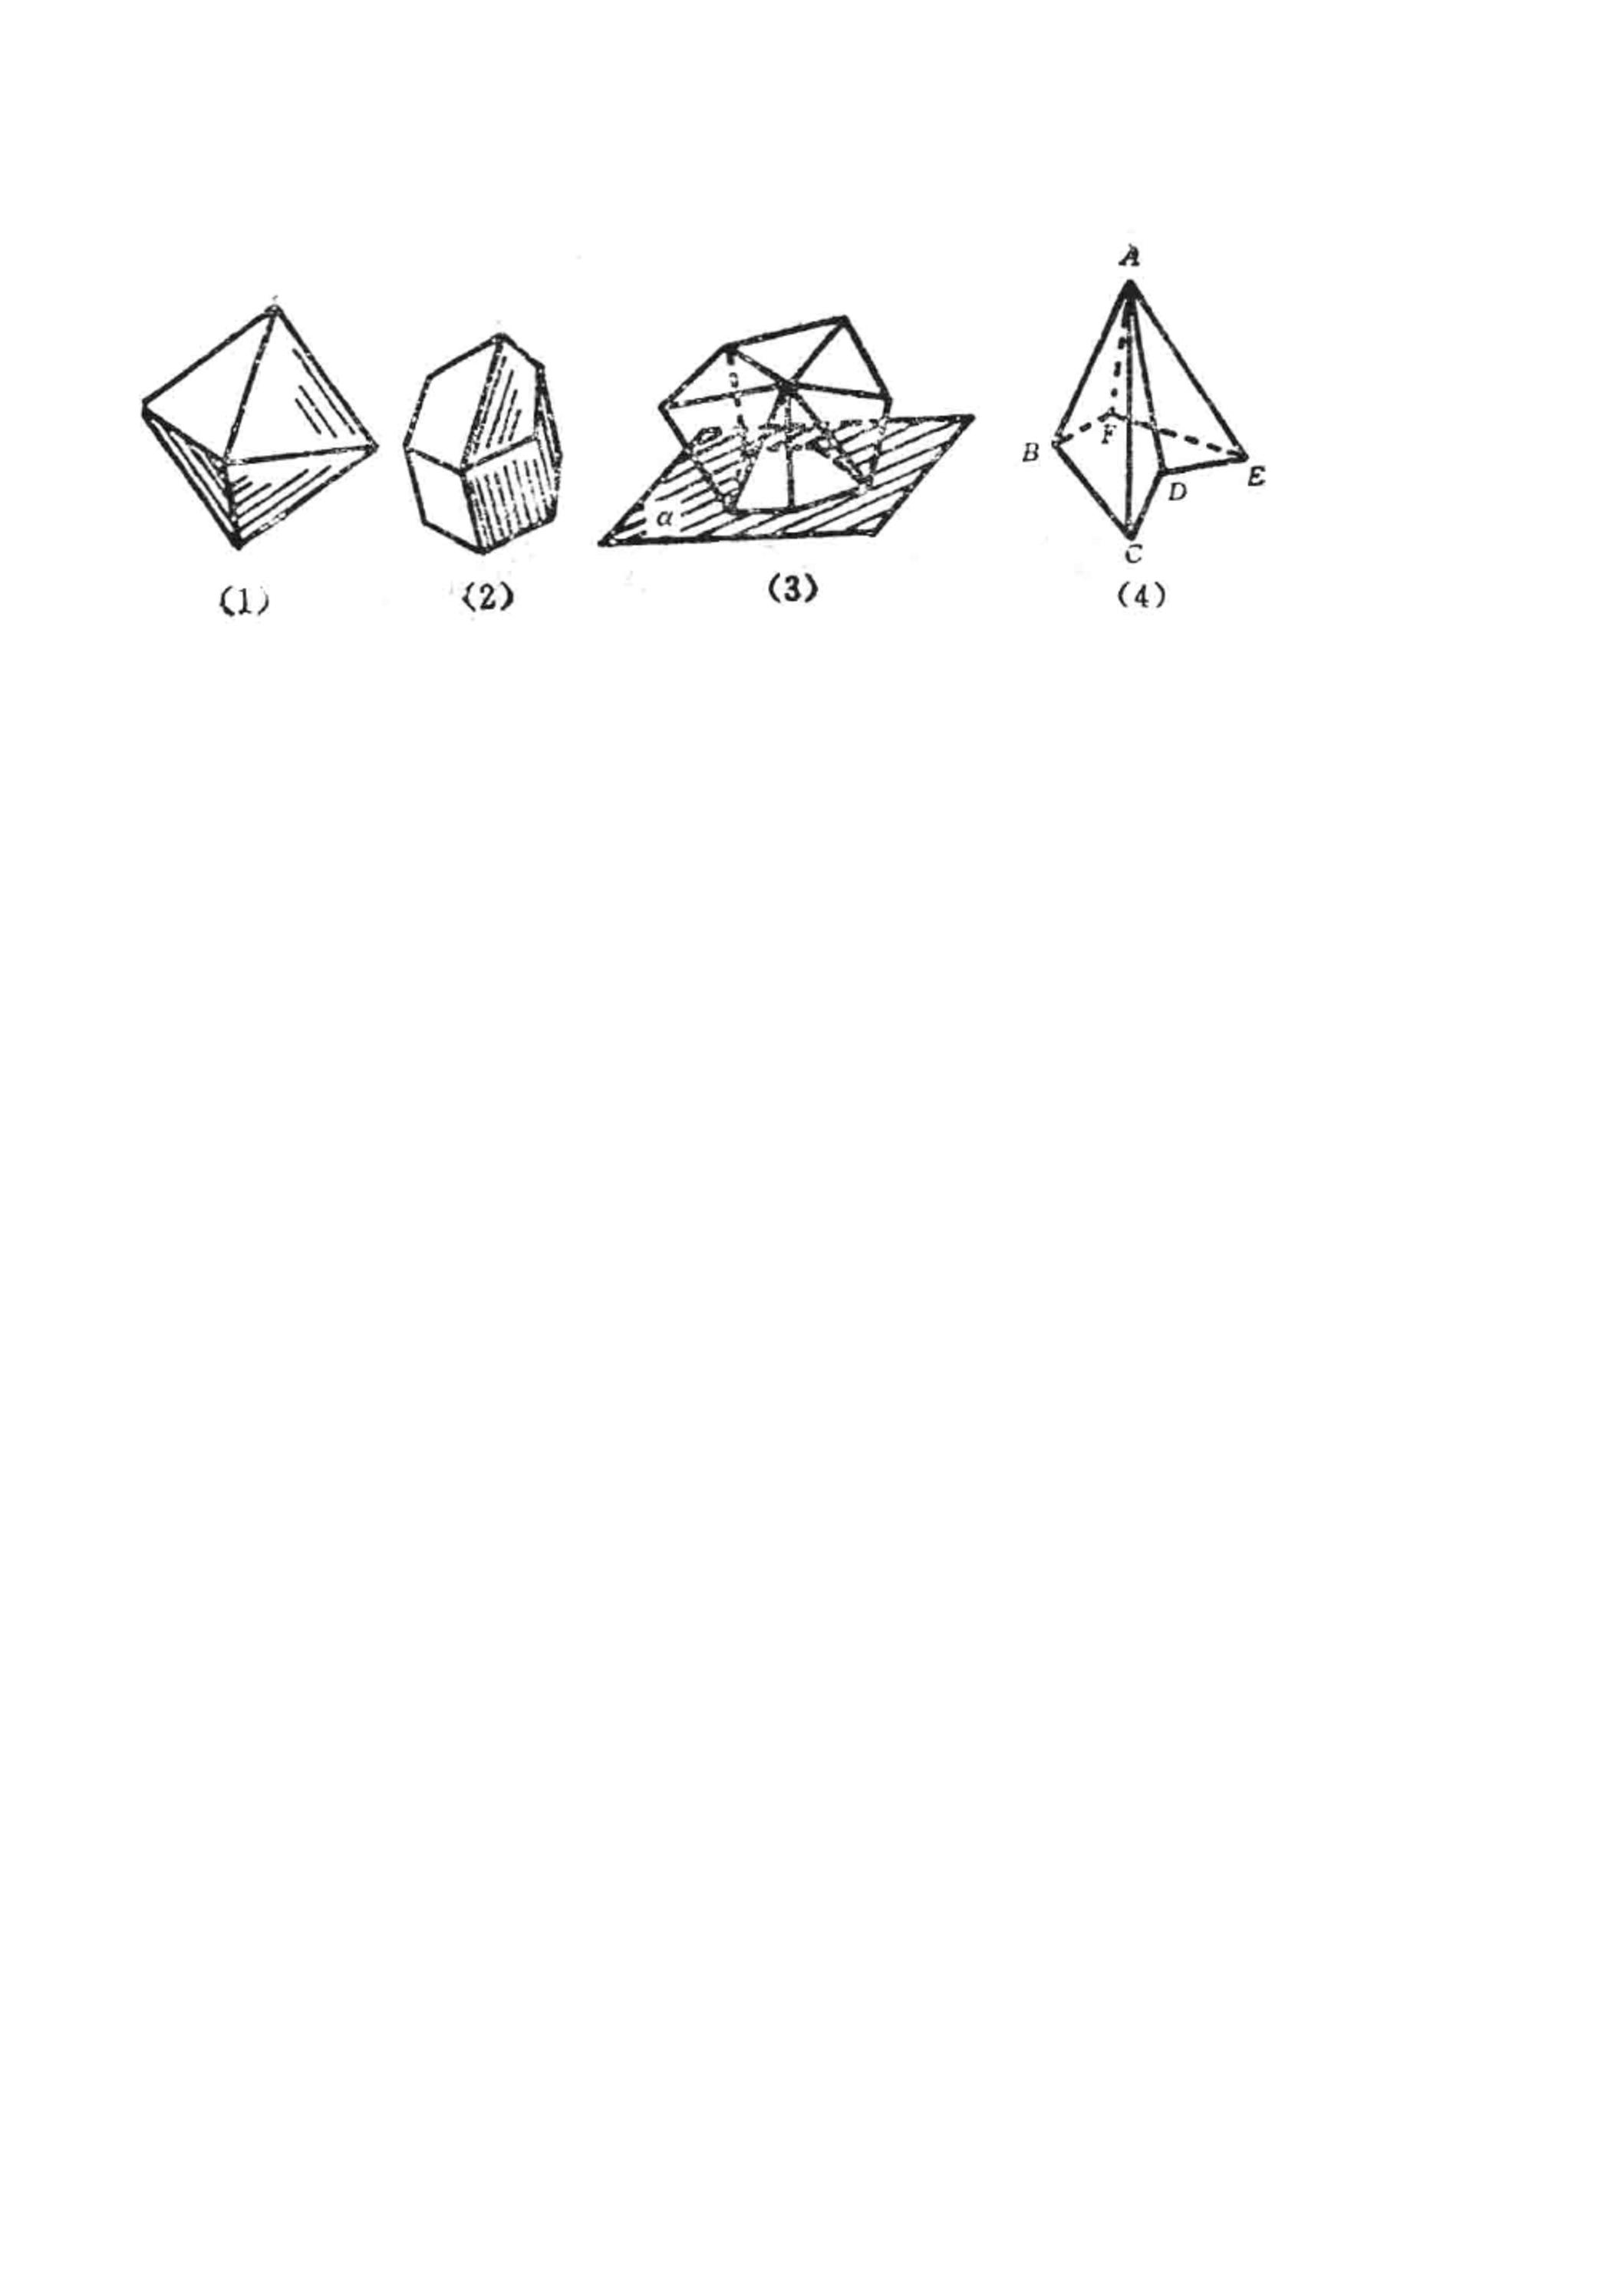
\includegraphics[scale=.4]{fig/2-1.pdf}
    \caption{}
\end{figure}

围成多面体的各个平面多边形，叫做\textbf{多面体的面}，每相邻两个面的公共边，叫做\textbf{多面体的棱}. 棱和棱的公共端点叫做\textbf{多面体的顶点}，连结不在多面体的同一面上的两个顶点的线段叫做\textbf{多面体的对角线}.

如果多面体对它的每一个面而言，都在该面所在平面的同侧，那么这类多面体叫做\textbf{凸多面体}．如图2.1中的（1）、（2）、（3）都是凸多面体，而（4）就不是凸多面体．本教材研究的多面体，只限于凸多面体.并且以后说到多面体时，都是指凸多面体而言.

一个多面体至少有四个面，多面体按照它的面的个数分别叫做\textbf{四面体}、\textbf{五面体}、\textbf{六面体}等等.

多面体用表示它的各顶点的字母来表示，如图2.1的（4）中的多面体，记作多面体$ABCDEF$.

\subsection{多面体的表面展开图}
把多面体沿着若干条棱剪开后，多面体的各面就可展在一个平面上，得到一个平面多边形，这个平面多边形就叫做这个多面体的表面展开图.

由于剪开的棱的不同，同一个多面体的表面展开图可以
不是全等形. 但是，无论怎样剪法，同一个多面体的表面展开图的面积是一样的.

\noindent
\begin{minipage}{.45\textwidth}\centering
\begin{tikzpicture}[scale=.7]
\tkzDefPoints{0/0/A, 2/0/B, 2.71/.71/C, .71/.71/D, 0/2/A'}
\foreach \x in {B,C,D}
{
\tkzDefPointBy[translation = from A to A'](\x) \tkzGetPoint{\x'}
}
\tkzDrawPolygon(A,B,C,C',D',A')
\tkzDrawSegments[dashed](A,D C,D D,D') 
\tkzDrawSegments[thick](A',B' B',C' B',B) 
\tkzLabelPoints[left](A',D',A,D)
\tkzLabelPoints[right](B,C,B',C')
\end{tikzpicture}
\captionof{figure}{}
\end{minipage}
\hfill
\begin{minipage}{.53\textwidth}
\centering
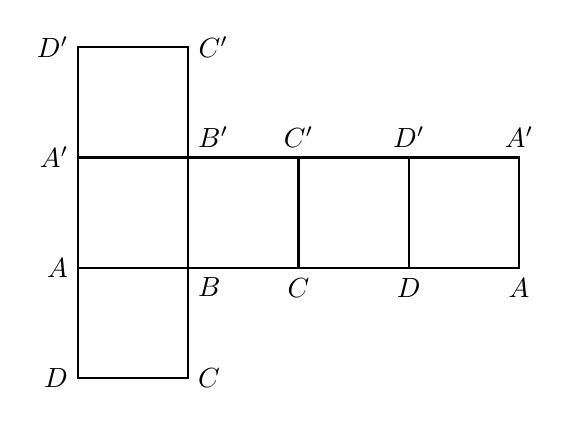
\begin{tikzpicture}[scale=1.4]
    \draw[thick](0,-1)node[left]{$D$} rectangle (1,2)node[right]{$C'$};
    \draw[thick](0,0)node[left]{$A$} rectangle(4,1);
    \draw[thick](2,0)node[below]{$C$}--(2,1)node[above]{$C'$};
    \draw[thick](3,0)node[below]{$D$}--(3,1)node[above]{$D'$};
    \draw[thick](4,0)node[below]{$A$}--(4,1)node[above]{$A'$};
    \node at (0,1)[left]{$A'$};
    \node at (0,2)[left]{$D'$};
    \node at (1,-1)[right]{$C$};
    \node at (1,0)[below right]{$B$};
    \node at (1,1)[above right]{$B'$};
    \end{tikzpicture}
\captionof{figure}{}
\end{minipage}

例如：图2.2是正方体，图2.3是它的一个表面展开图；图2.4是正方形，图2.5是正方体中过$A'$、$B'$、$C'$三点的平面切下的一个角的表面展开图.

图2.5中的展开图是沿多面体$B'A'BC'$中的棱$B'A'$, $BB'$和$B'C'$剪开的.



\subsection*{2.1 练习1}
画出长是5，宽是4，高是3的长方体的一个表面展开图。


\noindent
\begin{minipage}{.45\textwidth}
\centering\begin{tikzpicture}
    \tkzDefPoints{0/0/A, 2/0/B, 2.71/.71/C, .71/.71/D, 0/2/A'}
    \foreach \x in {B,C,D}
    {
    \tkzDefPointBy[translation = from A to A'](\x) \tkzGetPoint{\x'}
    }
    \tkzDrawPolygon(A,B,C,C',D',A')
    \tkzDrawSegments[dashed](A,D C,D D,D') 
    \tkzDrawSegments[thick](A',B' B',C' B',B A',C' A',B B,C') 
    \tkzLabelPoints[left](A',D',A,D)
    \tkzLabelPoints[right](B,C,B',C')
    \end{tikzpicture}
    \captionof{figure}{}
\end{minipage}
\hfill
\begin{minipage}{.53\textwidth}
\centering
\begin{tikzpicture}[]
    \tkzDefPoint(30:1.63){C'}
    \tkzDefPoint(150:1.63){A'}
    \tkzDefPoint(-90:1.63){B}
    \tkzDrawPolygon(A',B,C')
    \tkzDefPoint(90:2.23){B'_1}
    \tkzDefPoint(210:2.23){B'_2}
    \tkzDefPoint(-30:2.23){B'_3}
    \tkzDrawPolygon(B'_1,A',B'_2,B,B'_3,C')
    
    \tkzLabelPoints[above](B'_1)
    \tkzLabelPoints[below](B)
    \tkzLabelPoints[left](A',B'_2)
    \tkzLabelPoints[right](B'_3,C')
    
    \tkzMarkRightAngles[size=.15](C',B'_1,A' A',B'_2,B B,B'_3,C')
\end{tikzpicture}
\captionof{figure}{}
\end{minipage}



\subsection{多面体的截面}
一个平面截几何体，与几何体表面相交，由交线所围成的平面图形叫做这几何体的\textbf{截面}.

多面体的截面是一个平面多边形.画出多面体的截面就是画出这平面多边形的各边，要确定某个边所在的直线，只要知道这直线上的两个点.因此画多面体的截面关键是找截多面体的平面与多面体的面的公共点问题.

\begin{example}
        已知正方体$AC'$（如图2.6），$E$、$F$、$G$分别是$A'B'$、$B'B$、$B'C'$各棱的中点，求作过这三点的截面.
    \end{example}
    
    \begin{analyze}
    $\because\quad E$、$F$、$G$三点不共线，
    
    $\therefore\quad $它们确定一个平面$M$，要作出平面$M$和正方体某个面的交线，只要找到它们的两个公共点.
    \end{analyze}



\noindent
\begin{minipage}{.6\textwidth}\CTEXindent
    \begin{solution}
        \textbf{作法：}$E$、$F$是平面$M$与面$ABB'A'$的两个公共点，根据公理2，这两个面的交线是直线$EF$. 同理，直线$FG$、$GE$分别是平面$M$与平面$B'BCC'$
        和平面$A'B'C'D'$的交线. 从而线段$EF$、$FG$、$GE$所围成的三角形$EFG$就是所求作的截面.
        \end{solution}
\end{minipage}
\hfill
\begin{minipage}{.36\textwidth}
\centering
\begin{tikzpicture}[scale=1]
    \tkzDefPoints{0/0/A, 2/0/B, 2.71/.71/C, .71/.71/D, 0/2/A'}
    \foreach \x in {B,C,D}
    {
    \tkzDefPointBy[translation = from A to A'](\x) \tkzGetPoint{\x'}
    }
    \tkzDrawPolygon(A,B,C,C',D',A')
    \tkzDrawSegments[dashed](A,D C,D D,D') 
    \tkzDrawSegments[thick](A',B' B',C' B',B) 
    
    \tkzDefMidPoint(A',B')\tkzGetPoint{E}
    \tkzDefMidPoint(C',B')\tkzGetPoint{G}
    \tkzDefMidPoint(B,B')\tkzGetPoint{F}
    \tkzDrawPolygon[thick](E,F,G)
    \tkzLabelPoints[left](A',D',A,D,F)
    \tkzLabelPoints[right](B,C,C',G)
    \tkzLabelPoints[below](E)
    \tkzLabelPoints[below left](B')
\end{tikzpicture}
\captionof{figure}{}
\end{minipage}

\begin{example}
如图2.7，已知正方体$AC'$, $M\in B'C'$, $N\in B'B$, $K\in AD$，求作过$M$、$N$、$K$的截面.
\end{example}


\noindent
\begin{minipage}{.55\textwidth}\CTEXindent
\begin{analyze}
设截面为$\alpha$，我们就是要找到$\alpha$与正方体有关面的两个公共点，画出它们的交线. 正方体的各面在已知条件中只有面$B'BCC'$与截平面$\alpha$有两个公共点$M$、$N$.

$K$在面$A'ADD'$和面$ABCD$上，为了找到截面与这些面的另一公共点，我们还是要借助已知条件中给出的$M$、$N$的位置. 因为直线$MN$在面$BB'C'C$内，而平面$BB'C'C\cap$平面$ABCD=BC$，所以如果在$BC$上找到截面上的点就是找到了面$ABCD$与截面的公共点.显然这点就是直线$MN$与直线$BC$的交点$P$. 其余交点也可类似作出.
\end{analyze}
\end{minipage}
\hfill
\begin{minipage}{.43\textwidth}
\centering
\begin{tikzpicture}[scale=1.3]
\tkzDefPoints{0/0/A, 2/0/B, 2.71/.71/C, .71/.71/D, 0/2/A'}
\foreach \x in {B,C,D}
{
\tkzDefPointBy[translation = from A to A'](\x) \tkzGetPoint{\x'}
}
\tkzDrawPolygon(A,B,C,C',D',A')
\tkzDrawSegments[dashed](A,D C,D D,D') 
\tkzDrawSegments[](A',B' B',C' B',B) 
\tkzLabelPoints[left](A',D',A)
\tkzLabelPoints[right](B,C,C')
\tkzLabelPoints[below left](B')
\tkzLabelPoints[above right](D)
\tkzDefPointWith[linear, K=.6](A,D) \tkzGetPoint{K}
\tkzDefPointWith[linear, K=.3](C',B') \tkzGetPoint{M}
\tkzDefPointWith[linear, K=.2](B,B') \tkzGetPoint{N}
\tkzDefPointWith[linear, K=1.4](C,C') \tkzGetPoint{T'}
\tkzInterLL(M,N)(C,T')  \tkzGetPoint{T}
\tkzInterLL(M,N)(B,C)  \tkzGetPoint{P}

\tkzDrawSegments[](T,C' T,P) 


\tkzDrawLines[add= 0 and 0.1](T,P)
\tkzDrawLines[add= 0 and 0.6](C,B)

\tkzInterLL(P,K)(C,D)  \tkzGetPoint{Q}
\tkzInterLL(Q,T)(D',C')  \tkzGetPoint{W}
\tkzInterLL(Q,T)(A,A')  \tkzGetPoint{tmp1}

\tkzDrawPolygon[](T,W,M)
\tkzInterLL(P,K)(A,A')  \tkzGetPoint{tmp2}
\tkzDefPoints{0/.71/tmp3}
\tkzInterLL(P,Q)(A,B)  \tkzGetPoint{R}

\tkzDrawLines[add= 0 and 0.5](tmp1,Q  tmp2,Q tmp3,Q)
\tkzDrawSegments[dashed](tmp1,W D,tmp3 tmp2,R) 
\tkzDrawSegments[](R,P) 
\tkzLabelPoints[below](K,R)
\tkzLabelPoints[right](B,P,N,M)

\tkzDefPointBy[translation = from B to M](K) \tkzGetPoint{tmp4}
\tkzInterLL(tmp4,K)(T,Q)  \tkzGetPoint{S}
\tkzLabelPoints[above](Q,S,T,W)

\tkzDrawSegments[dashed](S,K) 
\tkzDrawSegments[very thick](N,R M,N W,M) 
\tkzDrawSegments[very thick, dashed](S,K S,W K,R) 
\end{tikzpicture}
\captionof{figure}{}
\end{minipage}

\begin{solution}
\textbf{作法：}
\begin{enumerate}[(1)]
\item 作直线$MN$，设$MN\cap BC=P$.
\item 连结$KP$，设$KP\cap AB=R$.
\item 延长$PK$和$CD$，设$PK\cap CD=Q$．又设$MN\cap $直线$C'C=T$，$QT\cap D'D=S$, $QT\cap D'C'=W$.
\item 连结$SK$、$WM$，则多边形$MNRKSW$就是所求作的截面.
\end{enumerate}
\end{solution}



\noindent
\begin{minipage}{.53\textwidth}\CTEXindent

\begin{example}
    已知正方体$AC'$中，$E\in C'D'$, $F\in C'C$, $K\in AB$，且$EC'=\frac{1}{3}C'D'$, $FC'=\frac{1}{3}CC'$, $AK=KB$，求作过$E$、$F$、$K$三点的截面.
\end{example}

\begin{analyze}
    如图2.8，连$EF$
    
$\because\quad $面$D'DCC'\parallel $面$A'ABB'$

$\therefore\quad $截面与它们的交线平行，

$\because\quad EF\parallel CD',\quad CD'\parallel A'B$, 从而有下面作法：
\end{analyze}
\end{minipage}
\hfill
\begin{minipage}{.45\textwidth}
\centering
\begin{tikzpicture}[scale=1.2]
    \tkzDefPoints{0/0/A, 2/0/B, 2.71/.71/C, .71/.71/D, 0/2/A'}
    \foreach \x in {B,C,D}
    {
    \tkzDefPointBy[translation = from A to A'](\x) \tkzGetPoint{\x'}
    }
    \tkzDrawPolygon(A,B,C,C',D',A')
    \tkzDrawSegments[dashed](A,D C,D D,D') 
    \tkzDrawSegments[](A',B' B',C' B',B) 
    \tkzLabelPoints[left](D',A)
    \tkzLabelPoints[right](C,C')
    \tkzLabelPoints[below left](B,B',A')
    \tkzLabelPoints[above left](D)
    
    \tkzDefPointWith[linear, K=0.333](C',D') \tkzGetPoint{E}
    \tkzDefPointWith[linear, K=0.333](C',C) \tkzGetPoint{F}
    \tkzDefMidPoint(A,B) \tkzGetPoint{K}
    \tkzDefMidPoint(A,A') \tkzGetPoint{P}
    
    
    
    \tkzInterLL(P,K)(B,B')  \tkzGetPoint{Q}
    \tkzInterLL(B',A')(P,K)  \tkzGetPoint{M}
    \tkzInterLL(B,C)(F,Q)  \tkzGetPoint{R}
    \tkzInterLL(D',A')(E,M)  \tkzGetPoint{N}
    \tkzLabelPoints[below](K,M,Q)
    \tkzLabelPoints[above](E)
    \tkzLabelPoints[right](F,R)
    \tkzLabelPoints[left](P,N)
    
    \tkzDrawLines[add= 0 and 0.5](P,M)
    \tkzDrawSegments[](B,A' Q,F Q,P B,Q  E,M A',M) % 
    \tkzDrawSegments[dashed](C,D' E,F K,R N,P) 
    
    \tkzDrawSegments[very thick](E,N F,R P,K) 
    \tkzDrawSegments[very thick, dashed](N,P E,F K,R) 
    
\end{tikzpicture}
\captionof{figure}{}
\end{minipage}




\begin{solution}
\textbf{作法：}
\begin{enumerate}[(1)]
\item 作$KP\parallel A'B$交$A'A$于$P$;
\item 设直线$PK\cap B'B=Q$, $PK\cap A'B'=M$;
\item 作直线$EM\cap A'D'=N$，直线$QF\cap BC=R$;
\item 连结$NP$、$KR$、$EF$，则多边形$EFRKPN$为所求作的截面.
\end{enumerate}
\end{solution}

\begin{remark}
    用例2.2的方法同样可作出这个截面，那就要首先找出直线$EF$与$DC$、$DD'$的交点.
\end{remark}

\begin{example}
    如图2.9，已知多面体$ABCDE$, $P\in ED$, $Q\in CD$, 求作过$PQ$而平行于$AB$的截面.
\end{example}

\begin{analyze}
    因为所作的截面要平行于$AB$，则$AB$一定要平行这截面中的某一条直线. 只要作出这条直线，截面就可确定.
    
    $\because\quad AB\subset $平面$ABD$，而$PQ\cap $平面$ABD=K$，$K$在截面中，过$K$作平行于$AB$的直线$KM$. 设$KM\cap AD=M$，从而得到截面三角形$MPQ$.
\end{analyze}


\noindent
\begin{minipage}{.52\textwidth}\CTEXindent
\begin{solution}
\textbf{作法：}
\begin{enumerate}[(1)]
\item 连结$BD$、$PQ$设$BD\cap  PQ=K$.
\item 过$K$作$KM\parallel AB$交$AD$于$M$.
\item 连结$PM$、$MQ$，则三角形$MPQ$为所求作的截面． 
\end{enumerate}
\end{solution}
\end{minipage}
\hfill
\begin{minipage}{.45\textwidth}
\centering
\begin{tikzpicture}[]
    \tkzDefPoints{0/0/B, 3.5/0/C, 4.5/1.5/D, 1/1.5/E, 3/3/A}
    \tkzDrawPolygon[thick](A,E,B,C,D)
    \tkzDrawSegments[dashed](D,E B,D) 
    \tkzDrawSegments[thick](A,C A,B) 
    \tkzLabelPoints[above](A)
    \tkzLabelPoints[right](D,C)
    \tkzLabelPoints[left](B,E)
    \tkzDefPointWith[linear, K=.45](D,E) \tkzGetPoint{P}
    \tkzDefPointWith[linear, K=.45](C,D) \tkzGetPoint{Q}
    \tkzInterLL(B,D)(P,Q)  \tkzGetPoint{K}
    \tkzDefPointBy[translation = from B to K](A) \tkzGetPoint{A'}
    \tkzInterLL(K,A')(A,D)  \tkzGetPoint{M}
    
    \tkzDrawSegments[dashed](P,M M,K P,Q) 
    \tkzDrawSegments[thick](M,Q) 
    \tkzLabelPoints[right](M,Q)
    \tkzLabelPoints[above](P)
    \tkzLabelPoints[below left](K)
\end{tikzpicture}
\captionof{figure}{}
\end{minipage}

\subsection*{2.1 练习2}
\begin{enumerate}
\item 为什么一个多面体至少有四个面？
\item 画出若干个凸多面体，数出它们的顶点数、棱数和面的个数。对任何凸多面体来说，这三个数之间有着一种固
定的关系，你能找出这个关系吗？（提示：计算：顶点数$+$面数$-$棱数$=?$）
\item 如果用一个平面去截正方体，截面可能是几边形？
\end{enumerate}

\section*{习题一}
\begin{center}
    \bfseries A
\end{center}

\begin{enumerate}
    \item 用较硬的纸按下图的样子按$1:5$的比例尺画好，剪下．再把它沿虚线折起来粘好（阴影部分粘合），做成多面体模型.
\begin{center}
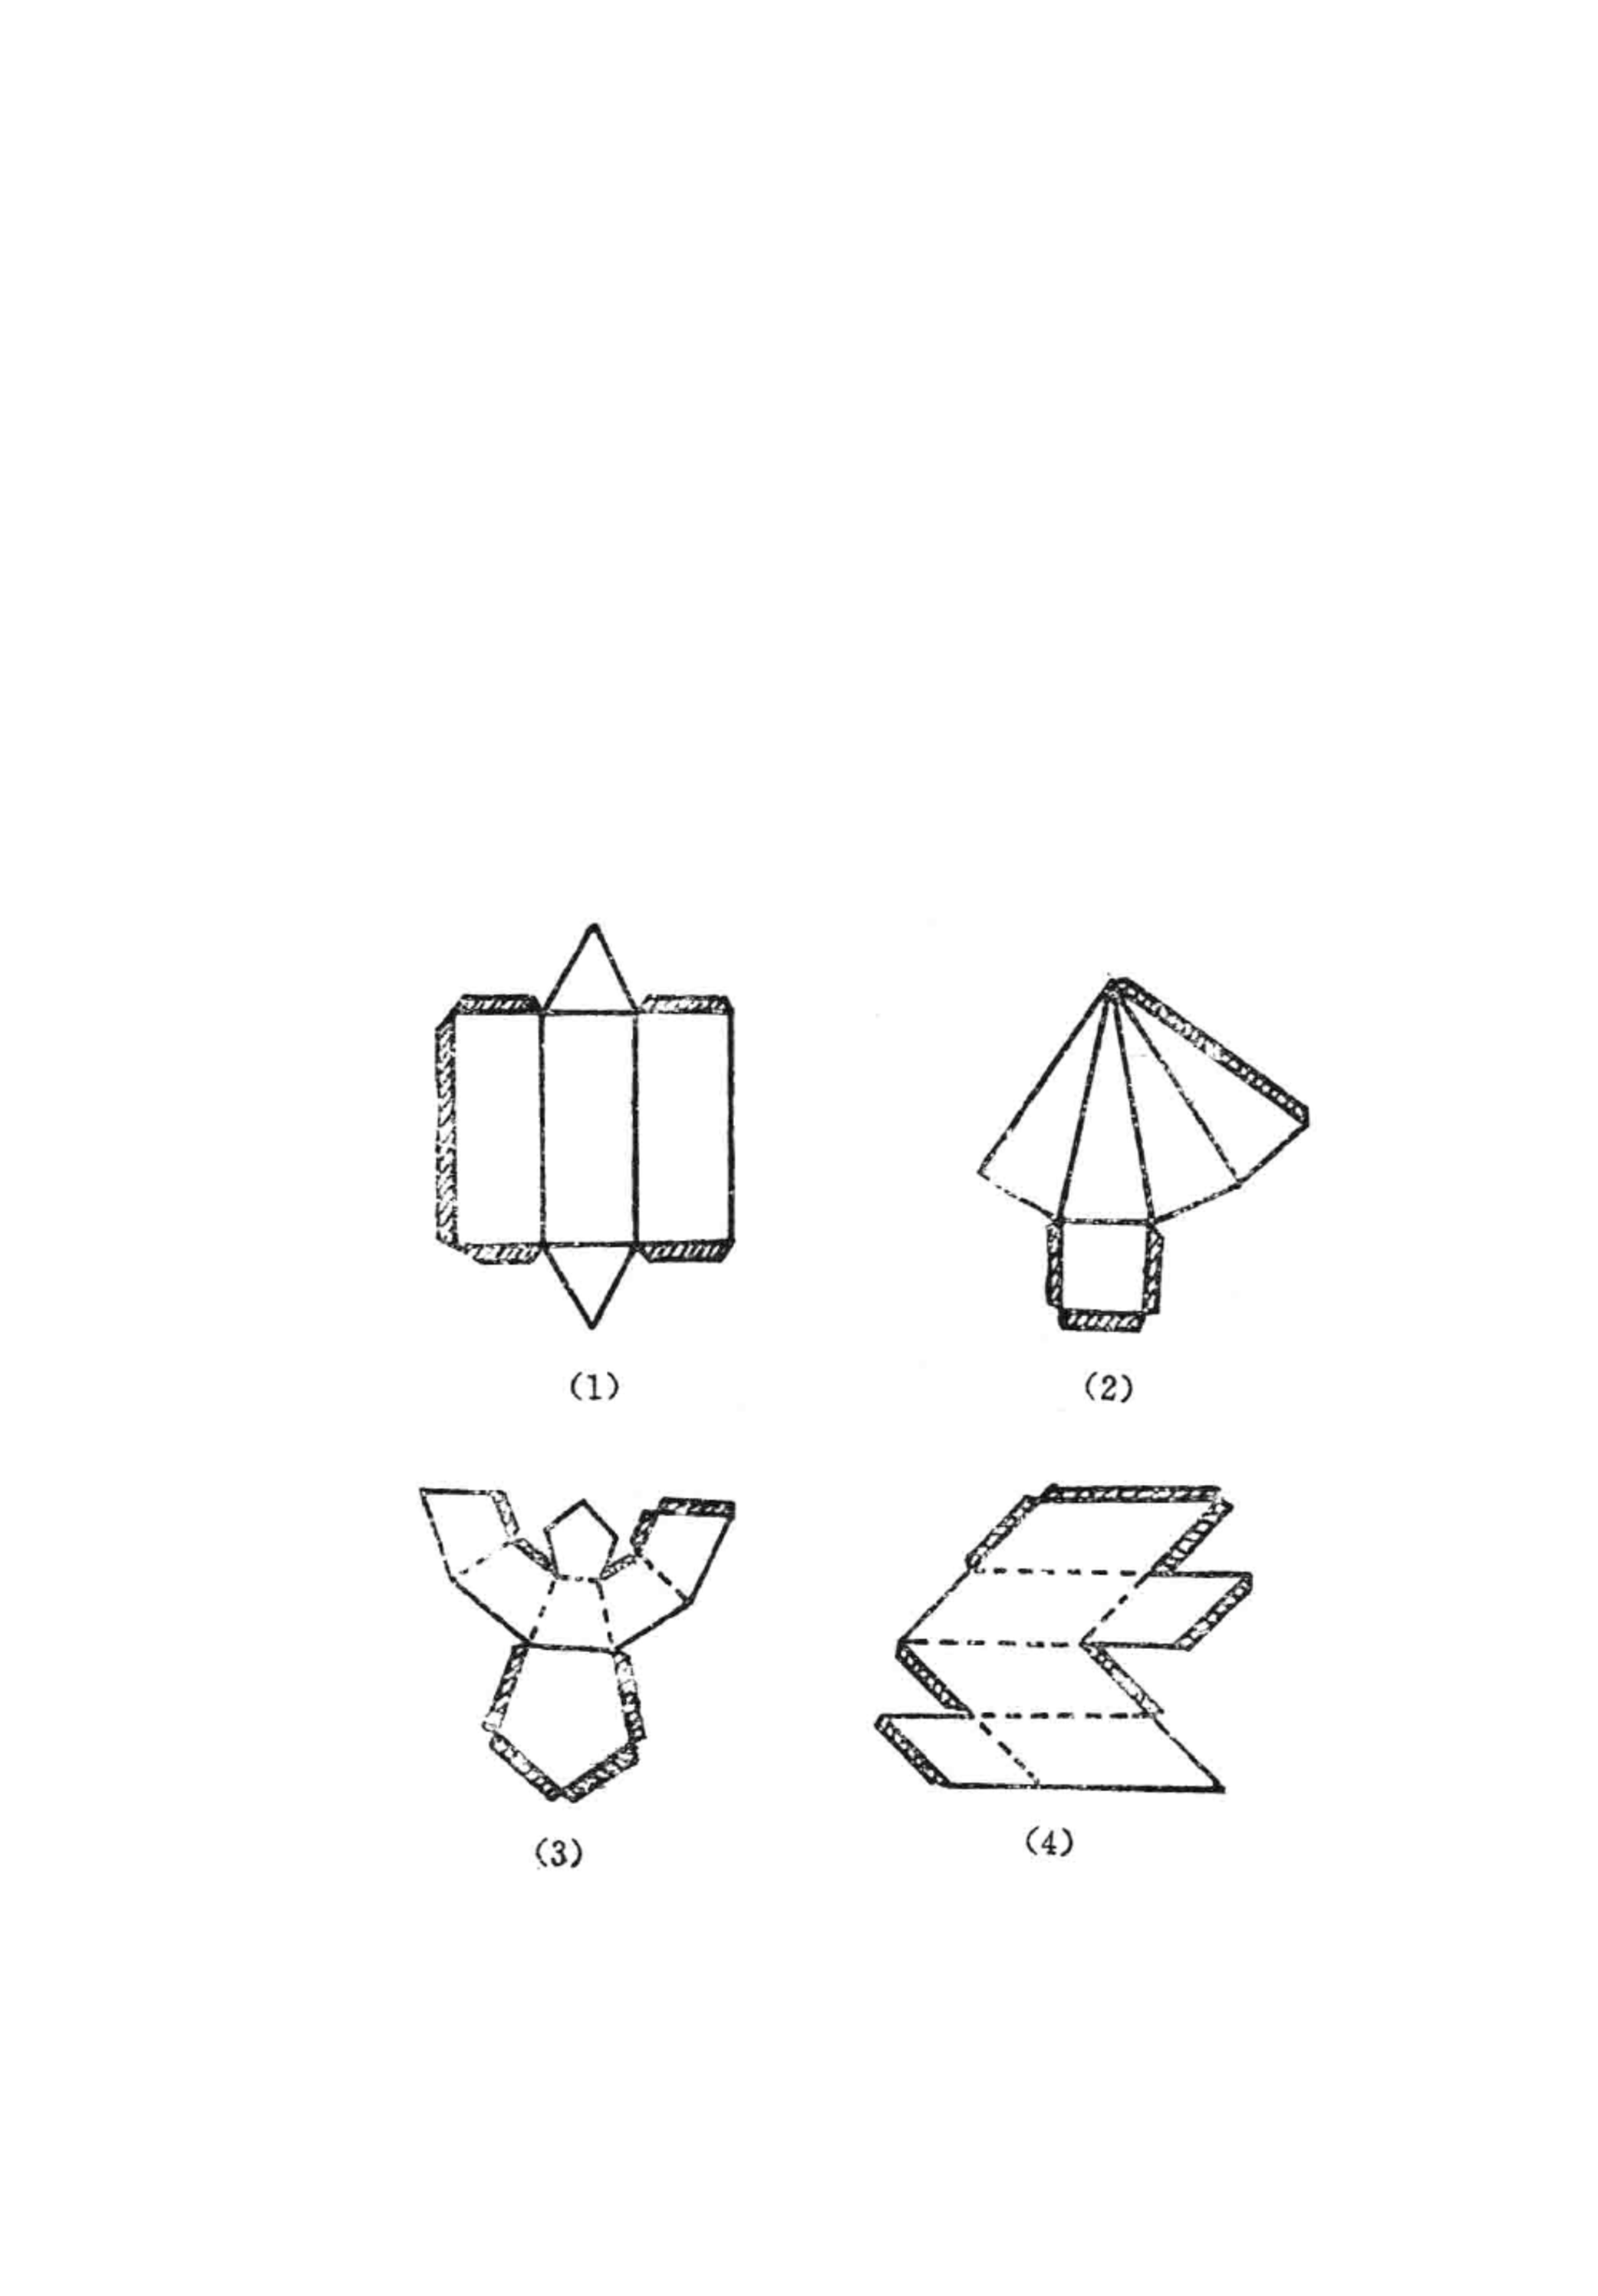
\includegraphics[scale=.4]{fig/2-ex1.pdf}
    \captionof*{figure}{第1题}
\end{center}

\item 如图，已知长方体$ABCD-A'B'C'D'$，按下列要求画出
它的表面展开图

\noindent
\begin{minipage}{.45\textwidth}
    \begin{enumerate}[(1)]
        \item 剪开棱$AB$、$AD$、$AA'$、$A'D'$、$BC$、$BB'$、$B'C'$;
        \item 剪开棱$AB$、$A'B'$、$AA'$、$BC$、$B'C'$、$AD$、$A'D'$;
        \item 剪开棱$AA'$、$A'B'$、$DD'$、$A'D'$、$BB'$、$CC'$、$C'D'$.
        \end{enumerate}
\end{minipage}
\hfill
\begin{minipage}{.45\textwidth}
\centering
\begin{tikzpicture}[]
    \tkzDefPoints{0/0/A, 3/0/B, 3.71/.71/C, 0/1.5/A'}
    \tkzDefPointBy[translation = from B to C](A) \tkzGetPoint{D}
    \foreach \x in {B,C,D}
    {
        \tkzDefPointBy[translation = from A to A'](\x) \tkzGetPoint{\x'}
    }
    
    \tkzDrawPolygon[thick](A,B,C,C',D',A')
    \tkzDrawSegments[dashed](A,D D,D' D,C) 
    \tkzDrawSegments[thick](A',B' B',C' B,B') 
    \tkzLabelPoints[right](B,C,B',C')
    \tkzLabelPoints[left](A,D,A',D')
    \end{tikzpicture}
    \captionof*{figure}{第2题}
\end{minipage}
\end{enumerate}

\begin{center}
    \bfseries B
\end{center}

\begin{enumerate}\setcounter{enumi}{2}
    \item 已知正方体$ABCD-A'B'C'D'$，画出符合下列条件的截面，$E$、$F$分别是$AB$、$BC$的中点：
\begin{multicols}{2}
   \begin{enumerate}[(1)]
\item 过$D_1$、$E$、$F$作截面；
\item 过$E$、$F$和$DD_1$的中点$M$;
\item 过点$E$和棱$A'D'$;
\item 过点$F$和棱$A'D'$;
\item 过$E$、$F$和$A'$;
\item 过$E$、$F$和$C'C$的中点$N$．
\end{enumerate} 
\end{multicols}


    \item 已知多面体$S-ABCD$，面$ABCD$是正方形，$SA=SB=SC=SD$, $P\in BS$, $Q\in BC$：
\begin{enumerate}[(1)]
    \item 过$PQ$作平行于$AB$的截面；
    \item  过$PQ$作垂直于面$ABCD$的截面.
\end{enumerate}
\end{enumerate}


\noindent
\begin{minipage}{.45\textwidth}
    \centering
\begin{tikzpicture}
\tkzDefPoints{0/0/A, 2/0/B, 2.71/.71/C, 0/2/A'}
\tkzDefPointBy[translation = from B to C](A) \tkzGetPoint{D}
\foreach \x in {B,C,D}
{
    \tkzDefPointBy[translation = from A to A'](\x) \tkzGetPoint{\x'}
}

\tkzDrawPolygon[thick](A,B,C,C',D',A')
\tkzDrawSegments[dashed](A,D D,D' D,C) 
\tkzDrawSegments[thick](A',B' B',C' B,B') 
\tkzLabelPoints[right](B,C,B',C')
\tkzLabelPoints[left](A,D,A',D')
\tkzDefMidPoint(D,D') \tkzGetPoint{M}
\tkzDefMidPoint(B,C) \tkzGetPoint{F}
\tkzDefMidPoint(A,B) \tkzGetPoint{E}
\tkzDefMidPoint(C,C') \tkzGetPoint{N}
\tkzDrawPoints(M,N,E,F)
\tkzLabelPoints[right](M,N,F)
\tkzLabelPoints[below](E)
\end{tikzpicture}
\captionof*{figure}{第3题}
\end{minipage}
\hfill
\begin{minipage}{.45\textwidth}
\centering
\begin{tikzpicture}[scale=1.4]
    \tkzDefPoints{0/0/A, 2/0/B, 3/1/C, 1.5/2.3/S}
    \tkzDefPointBy[translation = from B to C](A) \tkzGetPoint{D}
    \tkzDrawPolygon[thick](A,B,C,S)
    \tkzDrawSegments[dashed](S,D D,A D,C) 
    \tkzDrawSegments[thick](S,B) 
    \tkzDefPointWith[linear, K=.3](S,B) \tkzGetPoint{P}
    \tkzDefPointWith[linear, K=.4](C,B) \tkzGetPoint{Q}
    \tkzLabelPoints[right](B,C,Q)
    \tkzLabelPoints[left](A,P)
    \tkzLabelPoints[above](S)
    \tkzLabelPoints[below](D)
    \tkzDrawSegments[thick](S,B P,Q) 
    \end{tikzpicture}
    \captionof*{figure}{第4题}
\end{minipage}

\section{棱柱}
\subsection{棱柱的概念和性质}
一个多面体，如果有两个面互相平行，而其余各面都是四边形，并且每相邻两个四边形的公共边都互相平行，这样的多面体叫做\textbf{棱柱}（图2.10）．这两个互相平行的面叫做棱柱
的\textbf{底面}，简称\textbf{底}；而其余各面叫做\textbf{棱柱的侧面}；两个侧面的公共边叫做\textbf{棱柱的侧棱}；两个底面所在平面的公垂线段叫做\textbf{棱柱的高}（两个底面间的距离也简称高）. 过棱柱的不相邻两侧棱的截面叫做棱柱的对角面．如图2.10中的棱柱，多边形$ABCDE$和$A'B'C'D'E'$是底面，四边形$ABB'A'$, $BCC'B'$等是侧面，$A'A$、$B'B$等是侧棱，$H'H$是高，截面$B'BDD'$是对角面. 
\begin{figure}[htp]
    \centering
\begin{tikzpicture}
\tkzDefPoints{0/0/B, 1.5/0/C, 2.5/.6/D, 1.2/1.5/E, -.5/.5/A, .3/3/B'}
\foreach \x in {A,C,D,E}
{
    \tkzDefPointBy[translation= from B to B'](\x)
    \tkzGetPoint{\x'}
}
\tkzDrawPolygon[thick](A,B,C,D,D',E',A')
\tkzDrawSegments[thick](A',B' B',C' C',D' B,B' C,C')
\tkzDrawSegments[dashed](A,E E,D B,D C,E' E,E')


\tkzDefPoints{.8/.6/H, .7/3.5/H'}
\tkzDrawSegments[dashed](H,H' E',C)

\tkzLabelPoints[below](B,C,E)
\tkzLabelPoints[above](E',D',H')
\tkzLabelPoints[left](A,A',B',H)
\tkzLabelPoints[right](D,C')
\tkzDrawSegments[very thick](B',D')

\draw(D')--+(1,0)node[right]{棱柱的顶点};
\draw(2.3,2.5)--+(1,0)node[right]{棱柱的侧面};
\draw(2.52,1)--+(.5,0)node[right]{棱柱的侧棱};

\draw(.75,2.05)--+(-1.5,0)node[left]{棱柱的高};

\tkzDefPointWith[linear , K=.425](E',C) \tkzGetPoint{TMP1}
\draw(TMP1)--+(-2,0)node[left]{棱柱的对角线};

\draw(.5,.3)--+(-1.5,0)node[left]{棱柱的底面};
\draw(.5,3.5)--+(-2,.75)node[above]{棱柱的底面};
\end{tikzpicture}
    \caption{}
\end{figure}



棱柱用表示底面各顶点的字母来表示，如图2.2中的棱柱、记作棱柱$ABCDE-A'B'C'D'E'$，或者用表示一条对角线端点的两个字母来表示. 例如，棱柱$AC'$.

侧棱不垂直于底面的棱柱叫做\textbf{斜棱柱}（图2.10）；侧棱垂直于底面的棱柱叫做\textbf{直棱柱}（图2.11甲乙）．底面是正多边形的直棱柱叫做\textbf{正棱柱}（图2.11丙）．

棱柱的底面可以是三角形、四边形、五边形、……，我们把这样的棱柱分别叫做\textbf{三棱柱}（图2.11甲）、\textbf{四棱柱}（图2.11乙）、\textbf{五棱柱}（图2.11丙）、……

\begin{figure}[htp]
    \centering
\begin{tikzpicture}[scale=.8]
\begin{scope}
\tkzDefPoints{0/0/A, 2/.25/B, 1.5/-.5/C, 0/3/A'}
\foreach \x in {B,C}
{
    \tkzDefPointBy[translation= from A to A'](\x)
    \tkzGetPoint{\x'}
}
\tkzDrawPolygon(A,C,B,B',A')
\tkzDrawSegments[dashed](A,B)
\tkzDrawSegments(C,C' A',C' B',C')
\node at (1,-1){甲};
\end{scope}
\begin{scope}[xshift=4cm]    
\tkzDefPoints{0/0/A, 2/0/C, 1.25/-.8/B, 1/.5/D, 0/3/A'}
\foreach \x in {B,C,D}
{
    \tkzDefPointBy[translation= from A to A'](\x)
    \tkzGetPoint{\x'}
}
\tkzDrawPolygon(A,B,C,C',D',A')
\tkzDrawSegments[dashed](D,D' C,D D,A)
\tkzDrawSegments(B,B' B',C' A',B')
\node at (1,-1){乙};
\end{scope}
\begin{scope}[xshift=8cm]
\tkzDefPoints{0/-.5/A, 1.5/-.5/B, -.45/0/E, 1/.5/D, 2/0/C, 0/2.75/A'}
\foreach \x in {B,C,D,E}
{
    \tkzDefPointBy[translation= from A to A'](\x)
    \tkzGetPoint{\x'}
}
\tkzDrawPolygon(A,B,C,C',D',E',E)
\tkzDrawSegments[dashed](D,D' C,D E,D)
\tkzDrawSegments(B,B' A,A' A',B' B',C' E',A')
\node at (1,-1){丙};
\end{scope}
\end{tikzpicture}
    \caption{}
\end{figure}


根据棱柱的定义，容易得到棱柱具有下列性质：
\begin{enumerate}[(1)]
\item 棱柱的侧棱都相等，侧面是平行四边形；直棱柱的每个侧面都是矩形；正棱柱的各个侧面都是全等的矩形.

事实上，棱柱的每个侧面都具有两条平行的侧棱，又每个侧面与两个平行底面的交线互相平行（平行平面的性质），所以每个侧面是平行四边形，并且各条侧棱都相等，直棱柱的每条侧棱都垂直于底面，也就垂直于侧面与底面的交线. 由于有一个角是直角的平行四边形是矩形，所以直棱柱的侧面是矩形. 由于正棱柱的底面是正多边形，所以正棱柱的各个侧面是长宽分别相等的矩形，即它们是全等的矩形

\item 棱柱的两个底面与平行于底面的截面是全等的多边形（图2.12甲）．
\item 过棱柱的不相邻的两条侧棱的截面是平行四边形（图2.12乙）．
\end{enumerate}


\noindent
\begin{minipage}{.5\textwidth}
\centering
\begin{tikzpicture}[scale=.8]
\begin{scope}
\tkzDefPoints{0/-.5/A, 1.5/-.5/B, -.45/0/E, 1/.5/D, 2/0/C, 0/2.75/A'}
\foreach \x in {B,C,D,E}
{
    \tkzDefPointBy[translation= from A to A'](\x)
    \tkzGetPoint{\x'}
}
\tkzDrawPolygon(A,B,C,C',D',E',E)
\tkzDrawSegments[dashed](D,D' C,D E,D)
\tkzDrawSegments(B,B' A,A' A',B' B',C' E',A')

\foreach \x in {A,B,C,D,E}
{
    \tkzDefMidPoint(\x,\x')\tkzGetPoint{\x''}
}
\tkzDrawSegments[dashed](C'',D'' D'',E'')
\tkzDrawSegments(A'',B'' B'',C'' E'',A'')

\node at (1,-1){甲};
\end{scope}
\begin{scope}[xshift=4cm]
\tkzDefPoints{0/-.5/A, 1.5/-.5/B, -.45/0/E, 1/.5/D, 2/0/C, 0/2.75/A'}
\foreach \x in {B,C,D,E}
{
    \tkzDefPointBy[translation= from A to A'](\x)
    \tkzGetPoint{\x'}
}
\tkzDrawPolygon(A,B,C,C',D',E',E)
\tkzDrawSegments[dashed](D,D' C,D E,D A,C)
\tkzDrawSegments(B,B' A,A' A',B' B',C' E',A' A',C')
\node at (1,-1){乙};
\end{scope}
\end{tikzpicture}
\captionof{figure}{}
\end{minipage}
\hfill
\begin{minipage}{.45\textwidth}
\centering
\begin{tikzpicture}[scale=1.2]
\tkzDefPoints{0/0/A, 2/0/C, 1.35/.6/B, 0/2.5/A'}
\foreach \x in {B,C}
{
    \tkzDefPointBy[translation= from A to A'](\x)
    \tkzGetPoint{\x'}
}
\tkzDrawPolygon(A,C,C',B',A')
\tkzDrawSegments[dashed](A,B B,C B,B')
\tkzDrawSegments(A',C')

\tkzDefMidPoint(A',C')\tkzGetPoint{E}
\tkzDefMidPoint(B',C')\tkzGetPoint{F}
\tkzDefMidPoint(A',B')\tkzGetPoint{H}
\tkzDefMidPoint(B,A)\tkzGetPoint{G}
\tkzInterLL(C',H)(E,F)\tkzGetPoint{K}
\tkzDrawSegments[dashed](H,G B,F G,K)
\tkzDrawSegments(H,C' E,F A,E)

\tkzLabelPoints[above](B',K)
\tkzLabelPoints[below](E)
\tkzLabelPoints[left](A,A',H)
\tkzLabelPoints[right](C,G,C',F,B)

\end{tikzpicture}
\captionof{figure}{}
\end{minipage}

\begin{example}
    正三棱柱$ABC-A'B'C'$中，底面边长是$a$，侧棱长
    是$b$，$E$是$A'C'$的中点，求过$A$、$B$、$E$三点的截面的面积.
\end{example}

\begin{analyze}
过$A$、$B$、$E$三点的截面，就是$A$、$B$、$E$三点所确定的平面（因为它们不共线）与棱柱的某些面相交所得交线所围成的平面图形.因为棱柱各面都是平面图形，所以交线都是线段，截面是多边形. 只要求得截面多边形的各个顶点，截面就可作出. 因为棱柱上、下底面平行，所以截面在上、下底面中的两个边应该平行.
\end{analyze}

\begin{solution}
过$E$作$EF\parallel A'B'$交$B'C'$于$F$，连结$BF$、$AE$.

$\because\quad $面$ABC\parallel $面$A'B'C'$，则梯形$EFBA$是所求的截面.

取$AB$的中点$G$，$A'B'$的中点$H$，连结$HG$，则$HG\parallel A'A$，

$\therefore\quad HG\bot $平面$A'B'C'$，且$C'H\bot A'B'$.

$\therefore\quad EF\parallel A'B'$

$\therefore\quad C'H\bot EF$，设$EF\cap C'H=K$，由三垂线定理，
$EF\bot KG$，在${\rm Rt}\triangle GHK$中，$HG=AA'=b$，$E$是$A'C'$中点，$EF\parallel A'B'$

$\therefore\quad KH=\frac{1}{2}HC'=\frac{1}{2}\cdot \frac{\sqrt{3}}{2}a=\frac{\sqrt{3}}{4}a$
\[ \therefore\quad GK=\sqrt{GH^2+HK^2}=\sqrt{b^2+\left(\frac{\sqrt{3}}{4}a\right)^2}=\frac{1}{4}\sqrt{3a^2+16b^2}\]
\[\begin{split}
 \therefore\quad S_{EFBA}=\frac{1}{2}(AB+EF)\cdot KG &=\frac{1}{2}\left(a+\frac{1}{2}a\right)\cdot \frac{1}{4}\sqrt{3a^2+16b^2}\\
    &=\frac{3a}{16}\sqrt{3a^2+16b^2}
\end{split}\]
\end{solution}

\subsection*{2.2 练习1}
\begin{enumerate}
\item 一个多面体要是棱柱，它需具有哪些条件？如果把“每相邻的两个四边形的公共边都互相平行”这一条件去掉行不行？
\item 计算：
\begin{enumerate}[(1)]
\item 六棱柱对角面的个数；
\item 六棱柱对角线的条数。
\end{enumerate}
\end{enumerate}


\subsection{平行六面体}
现在研究四棱柱的特殊情形.
底面是平行四边形的四棱柱叫做\textbf{平行六面体}（图2.14甲）. 侧棱与底面垂直的平行六面体叫做\textbf{直平行六面体}（图2.14乙）．底面是矩形的直平行六面体叫做\textbf{长方体}（图2.14丙），棱长都相等的长方体叫做\textbf{正方体}（图2.14丁）.

\begin{figure}[htp]
    \centering
\begin{tikzpicture}[scale=.8]
    \begin{scope}[xshift=0cm]
\tkzDefPoints{0/0/A, 2/0/B, 2.8/.35/C, .8/2.5/A'}
\tkzDefPointBy[translation = from B to C](A) \tkzGetPoint{D}
\foreach \x in {B,C,D}
{
    \tkzDefPointBy[translation= from A to A'](\x)
    \tkzGetPoint{\x'}
}
\tkzDrawPolygon[](A,B,C,C',D',A')
\tkzDrawSegments(A',B' B',C' B,B')
\tkzDrawSegments[dashed](D,D' C,D D,A)
\node at (1.2,-.5){甲};
\end{scope}
\begin{scope}[xshift=4cm]
\tkzDefPoints{0/0/A, 2/0/B, 2.8/.35/C, 0/2.5/A'}
\tkzDefPointBy[translation = from B to C](A) \tkzGetPoint{D}
\foreach \x in {B,C,D}
{
    \tkzDefPointBy[translation= from A to A'](\x)
    \tkzGetPoint{\x'}
}
\tkzDrawPolygon[](A,B,C,C',D',A')
\tkzDrawSegments(A',B' B',C' B,B')
\tkzDrawSegments[dashed](D,D' C,D D,A)
\node at (1.2,-.5){乙};
\end{scope}
\begin{scope}[xshift=8cm]
\tkzDefPoints{0/0/A, 2/0/B, 2.71/.71/C, 0/2.5/A'}
\tkzDefPointBy[translation = from B to C](A) \tkzGetPoint{D}
\foreach \x in {B,C,D}
{
    \tkzDefPointBy[translation= from A to A'](\x)
    \tkzGetPoint{\x'}
}
\tkzDrawPolygon[](A,B,C,C',D',A')
\tkzDrawSegments(A',B' B',C' B,B')
\tkzDrawSegments[dashed](D,D' C,D D,A)
\node at (1.2,-.5){丙};

\end{scope}
\begin{scope}[xshift=12cm]
\tkzDefPoints{0/0/A, 2/0/B, 2.71/.71/C, 0/2/A'}
\tkzDefPointBy[translation = from B to C](A) \tkzGetPoint{D}
\foreach \x in {B,C,D}
{
    \tkzDefPointBy[translation= from A to A'](\x)
    \tkzGetPoint{\x'}
}
\tkzDrawPolygon[](A,B,C,C',D',A')
\tkzDrawSegments(A',B' B',C' B,B')
\tkzDrawSegments[dashed](D,D' C,D D,A)
\node at (1.2,-.5){丁};
\end{scope}
\end{tikzpicture}
    \caption{}
\end{figure}

容易证明平行六面体具有下列性质：
\begin{thm}{性质}
  平行六面体任何相对两面各为互相平行并且全等的平行四边形.  
\end{thm}


因此，平行六面体的任何相对的两个面，都可看作底面.另外根据长方体和正方体的定义可以得到，长方体的六个面都是矩形，正方体的六个面都是正方形.

\begin{thm}
  {定理} 长方体一条对角线长的平方等于一个顶点上三条棱的长的平方和.  
\end{thm}

 已知：长方体$AC'$中，$B'D$是一条对角线.

    求证：$B'D^2=AB^2+BC^2+{BB'}^2$.
    
    \begin{analyze}
        从已知和求证两方面来看，需要构成以$B'D$为斜边的直角三角形，这只要连出一条以$D$或$B'$为顶点的面的对角线即可.
    \end{analyze}


\begin{proof}
连结$DB$. 在长方体$AC'$中，$BB'\bot $平面$ABCD$, $DB\subset$平面$ABCD$.

\noindent
\begin{minipage}{.55\textwidth}\CTEXindent
$\therefore\quad BB'\bot DB$

$\therefore\quad B'D^2=DB^2+B'B^2$

又$ABCD$是矩形，

$\therefore\quad DB^2=AB^2+BC^2$,

$\therefore\quad B'D^2=AB^2+BC^2+{B'B}^2$.
\end{minipage}
\hfill
\begin{minipage}{.43\textwidth}
\centering
\begin{tikzpicture}[]
\tkzDefPoints{0/0/A, 3/0/B, 3.71/.71/C, 0/1.3/A'}
\tkzDefPointBy[translation = from B to C](A) \tkzGetPoint{D}
\foreach \x in {B,C,D}
{
    \tkzDefPointBy[translation= from A to A'](\x)
    \tkzGetPoint{\x'}
}
\tkzDrawPolygon[](A,B,C,C',D',A')
\tkzDrawSegments(A',B' B',C' B,B')
\tkzDrawSegments[dashed](D,D' C,D D,A B',D B,D)

\tkzLabelPoints[left](A,A',D',D)
\tkzLabelPoints[right](B,C,B',C')
\end{tikzpicture}
\captionof{figure}{}
\end{minipage}
\end{proof}



\begin{thm}
    {推论1} 长方体的四条对角线等长．
\end{thm}

 \begin{thm}   
{推论2} 棱长为$a$的正方体的对角线长是$\sqrt{3}a$.
\end{thm}


\noindent
\begin{minipage}{.5\textwidth}
\begin{example}
    长方体的一条对角线与一个顶点上的三条棱所成的角分别是$\alpha$、$\beta$、$\gamma$. 
    
    求证：$\cos^2\alpha+\cos^2\beta+\cos^2\gamma=1$
\end{example}

\begin{analyze}
只要用长方体的棱与对角线表示出$\cos\alpha$、$\cos\beta$、$\cos\gamma$，再用已学过的长方体的对角线与共顶点的三条棱长的关系即可证明.
\end{analyze}
\end{minipage}
\hfill
\begin{minipage}{.48 \textwidth}
\centering
\begin{tikzpicture}[]
\tkzDefPoints{0/0/A, 3 /0/B, 4/1/C, 0/2.25/A'}
\tkzDefPointBy[translation = from B to C](A) \tkzGetPoint{D}
\foreach \x in {B,C,D}
{
    \tkzDefPointBy[translation= from A to A'](\x)
    \tkzGetPoint{\x'}
}
\tkzDrawPolygon[](A,B,C,C',D',A')
\tkzDrawSegments(A',B' B',C' B,B' D',B' B',C A,B')
\tkzDrawSegments[dashed](D,D' C,D D,A B',D)

\tkzLabelPoints[left](A,A',D',D)
\tkzLabelPoints[right](B,C,B',C')

\tkzMarkAngles[size=.2, mark=none](A,D,B')
\tkzMarkAngles[size=.35, mark=none](B',D,D')
\tkzLabelAngle[pos=.4](A,D,B'){$\alpha$}
\tkzLabelAngle[pos=.5](B',D,D'){$\gamma$}
\tkzMarkAngles[size=.6, mark=none](C,D,B')
\tkzLabelAngle[pos=.8](C,D,B'){$\beta$}


\end{tikzpicture}
\captionof{figure}{}
\end{minipage}



\begin{proof}
连结$AB'$、$B'C$、$B'D'$

$\because\quad $在长方体$AC'$中，$\triangle B'DA$、$\triangle B'DC'$、$\triangle B'DD'$都是直角三角形.

$\therefore\quad \cos\alpha=\frac{DA}{DB'},\quad \cos\beta=\frac{DC}{DB'},\quad \cos\gamma=\frac{DD'}{DB'}$

把上述三个等式两边同时平方后相加，得
\[
\therefore\quad \cos^2\alpha+\cos^2\beta+\cos^2\gamma =\frac{DA^2+DC^2+{DD'}^2}{{DB'}^2}=\frac{{DB'}^2}{{DB'}^2}=1
\]
\end{proof}


\noindent
\begin{minipage}{.58\textwidth}
\begin{example}
    已知长方体$AC'$，$BC=a$，$BB'=b$，求棱$AB$与平
面$A'DCB'$的距离.
\end{example}

\begin{analyze}
由长方体的性质，可得：$AB\parallel $平面$A'C$，$AB\bot $平面$B'C$. 设平面$A'C\cap$平面$B'C=B'C$，则$B$点到$B'C$的距离即$AB$与面$A'C$的距离.
\end{analyze}

\end{minipage}
\hfill
\begin{minipage}{.4\textwidth}
\centering
\begin{tikzpicture}[]
\tkzDefPoints{0/0/A, 3/0/B, 3.71/.71/C, 0/1.5/A'}
\tkzDefPointBy[translation = from B to C](A) \tkzGetPoint{D}
\foreach \x in {B,C,D}
{
    \tkzDefPointBy[translation= from A to A'](\x)
    \tkzGetPoint{\x'}
}
\tkzDefPointWith[linear, K=.6](B',C) \tkzGetPoint{E} 


\tkzDrawPolygon[](A,B,C,C',D',A')
\tkzDrawSegments(A',B' B',C' B,B' B',C  B',C B,E)
\tkzDrawSegments[dashed](D,D' C,D D,A  A',D)

\tkzLabelPoints[left](A,A',D',D)
\tkzLabelPoints[right](B,C,B',C')
\tkzLabelPoints[above right=-.2](E)
\end{tikzpicture}
\captionof{figure}{}
\end{minipage}

\begin{solution}
$\because\quad AB\parallel A'B'$

$\therefore\quad AB\parallel $平面$A'DCB'$

$\therefore\quad AB$上各点到平面$A'DCB'$的距离相等.

$\because\quad $长方体中，$A'B'\bot $面$B'BCC'$. 而$A'B'\subset $平面$A'DCB'$

$\therefore\quad $平面$A'DCB'\bot $平面$B'BCC'$

作$BE\bot B'C$于$E$. 

$\because\quad$平面$A'DCB'\cap $平面$B'BCC'=B'C$，

$\therefore\quad BE\bot $平面$A'DCB'$，则$BE$是棱$AB$与平面$A'DCB'$的距离.

在${\rm Rt}\triangle B'BC$中，$BC=a$, $BB'=b$,

$\therefore\quad BE=\frac{BB'\cdot BC}{B'C}=\frac{ab}{\sqrt{a^2+b^2}}$
\end{solution}

\begin{rmk}
    由例2.7可知，$AB$与平面$A'DCB'$的距离即异面直线$AB$、$A'C$的距离.
\end{rmk}



\noindent
\begin{minipage}{.55\textwidth}
    \begin{example}
        正方体$AC'$中，棱长为$a$.
    \begin{enumerate}[(1)]
    \item 求证：$D'B\bot $平面$B'AC$.
    \item 平面$B'AC$分$BD'$为$1:2$两部分．
    \end{enumerate}
    
    \end{example}
\end{minipage}
\hfill
\begin{minipage}{.4\textwidth}
\centering
\begin{tikzpicture}[]
\tkzDefPoints{0/0/A, 2/0/B, 2.71/.6/C, 0/2/A'}
\tkzDefPointBy[translation = from B to C](A) \tkzGetPoint{D}
\foreach \x in {B,C,D}
{
    \tkzDefPointBy[translation= from A to A'](\x)
    \tkzGetPoint{\x'}
}

\tkzDrawPolygon[](A,B,C,C',D',A')
\tkzDrawSegments(A',B' B',C' B,B' B',C    B',D'  A,B')
\tkzDrawSegments[dashed](D,D' C,D D,A  A,C B,D B,D')

\tkzLabelPoints[left](A,A',D',D)
\tkzLabelPoints[right](B,C,B',C')

\tkzInterLL(A,C)(B,D) \tkzGetPoint{O}
\tkzInterLL(B,D')(B',O) \tkzGetPoint{H}
\tkzDrawSegments[dashed](B',O)
\tkzLabelPoints[right](H)
\tkzLabelPoints[below](O)

\end{tikzpicture}
\captionof{figure}{}
\end{minipage}


\begin{analyze}
\begin{enumerate}[(1)]
    \item 只要证明$D'B$垂直于平面$AB'C$内的两条相交直线. 由正方体性质易知$D'D\bot $平面$AC$，且$AC\bot DB$. 由三垂线定理易证$D'B\bot AC$，同理可证$D'B\bot B'C$.
    \item 必须求出$BD'$与平面$B'AC$的交点，这只要找出含有$D'B$的平面与平面$B'AC$的交线即可. 这交线与$D'B$的交点即是所求的点.
\end{enumerate} 
\end{analyze}

\begin{proof}
\begin{enumerate}[(1)]
    \item 正方体$AC'$中，$D'D\bot $平面$ABCD$. $DB$是$D'B$
    在平面$ABCD$中的射影，而$ABCD$是正方形，$AC\bot BD$根据三垂线定理$AC\bot D'B$.

    同理$B'C\bot D'B$, 而$B'C\cap AC=C$ 
    
    $\therefore\quad D'B\bot $平面$AB'C$.
  \item 设$AC\cap DB=O$，连结$D'B'$，则$D'B\subset $平面$D'DBB'$，
  
  $\therefore\quad O$点与$B'$点是平面$D'DBB'$与平面$AB'C$的两个公共点，
  
  $\therefore\quad $直线$OB'$是这两个面的交线，设$D'B\cap OB'=H$，则$H$是$D'B$与平面$AB'C$的交点.

  在$\triangle D'HB'$和$\triangle BHO$中，$OB\paraeq \frac{1}{2}D'B$.

$\therefore\quad  \frac{BH}{HD'}=\frac{OB}{D'B'}=\frac{1}{2}$
    即平面$B'AC$分$BD'$为$1:2$两部分．
\end{enumerate}
\end{proof}

\begin{remark}
联系此例（1）（2）两个结论，可推得下述结果：
\begin{enumerate}
\item 点$B$到平面$AB'C$的距离是$\frac{\sqrt{3}}{3}a$.
\item 点$D'$到平面$A'DC'$的距离是$\frac{\sqrt{3}}{3}a$.
\item 平行平面$A'C'D$与$AB'C$的距离是$\frac{\sqrt{3}}{3}a$.
\item 异面直线$AC$与$A'D$的距离是$\frac{\sqrt{3}}{3}a$.
\item 二面角$B'-AC-B$的大小是$\arctan\sqrt{2}$.
\end{enumerate}
\end{remark}

\subsection*{2.2 练习2}

一、选择题（每题仅有一个正确答案）：
\begin{enumerate}
    \item 在下列条件中使图形为长方体的是\hfill    (\qquad)
    \begin{enumerate}[(A)]
    \item 侧面都是矩形的四棱柱。
    \item 对角面是矩形的四棱柱.
    \item 对角线相等的平行六面体.
    \item 底面是矩形，并且有两个侧面是矩形的四棱柱.
    \end{enumerate}

    \item 设$M=\{\text{正方体}\}$, $N=\{\text{长方体}\}$，$P=\{\text{直四棱柱}\}$，$Q=\{\text{正四棱柱}\}$，则这些集合间的关系是\hfill    (\qquad)
\begin{multicols}{2}
    \begin{enumerate}[(A)]
\item $M\subset Q\subset N\subset P$.
\item $M\subset P\subset N\subset Q$.
\item $P\subset Q\subset N\subset M$.
\item $M\subset N\subset Q\subset P$.
\end{enumerate}
\end{multicols}


    \item 已知正三棱柱$ABC-A'B'C'$, $D'$为$A'C'$中点，$AB=\sqrt{3}$, $AA'=1$，异面直线$AD'$和$BB'$间的距离是\hfill    (\qquad)

    \noindent
    \begin{minipage}{.6\textwidth}
\begin{multicols}{2}
    \begin{enumerate}[(A)]
        \item $\frac{6}{5}$.
        \item $\frac{2\sqrt{21}}{7}$.
        \item $\frac{\sqrt{5}}{6}$.
        \item $\frac{3}{2}$.
        \end{enumerate}
\end{multicols}

\item 如图，正方体$ABCD-A'B'C'D'$中$E$是$BC$中点，平面$BDE$与平面$BB'C'C$所成二面角$\alpha$的三角函数值是
\hfill    (\qquad)
    \end{minipage}
    \hfill
    \begin{minipage}{.37\textwidth}
    \centering
    \begin{tikzpicture}[]
    \tkzDefPoints{0/0/A, 2/0/B, 2.6/.8/C, 0/2/A'}
\tkzDefPointBy[translation = from B to C](A) \tkzGetPoint{D}
\foreach \x in {B,C,D}
{
    \tkzDefPointBy[translation= from A to A'](\x)
    \tkzGetPoint{\x'}
}
\tkzDefMidPoint(B',C') \tkzGetPoint{E}
\tkzDrawPolygon[](A,B,C,C',D',A')
\tkzDrawSegments(A',B' B',C' B,B' B,E)
\tkzDrawSegments[dashed](D,D' C,D D,A  D,B E,D)
\tkzLabelPoints[left](A,A',D',D)
\tkzLabelPoints[above left](B')
\tkzLabelPoints[right](B,C,C')
\tkzLabelPoints[right=-.15](E)

    \end{tikzpicture}
    \captionof*{figure}{第4题}
    \end{minipage}

\begin{multicols}{2}
\begin{enumerate}[(A)]
    \item $\cot\alpha=\frac{2}{\sqrt{5}}$
    \item $\cos\alpha=\frac{2}{\sqrt{5}}$
    \item $\sin\alpha=\frac{1}{\sqrt{5}}$
    \item $\tan\alpha=2\sqrt{2}$
\end{enumerate}
\end{multicols}

\item 已知某正方体对角线长为a，那么这正方体的表面积是\hfill    (\qquad)
\begin{multicols}{4}
    \begin{enumerate}[(A)]
\item $2\sqrt{2}a^2$
\item $2a^2$
\item $2\sqrt{3}a^2$
\item $3\sqrt{2}a^2$
\end{enumerate}
\end{multicols}
\end{enumerate}

二、填空题：
\begin{enumerate}\setcounter{enumi}{5}
\item 若长方体的一条对角线与一个顶点上的三条棱所成的角分别是$\alpha,\beta,\gamma$，则
\begin{enumerate}[(1)]
\item $\cos^2\alpha+\cos^2\beta+\cos^2\gamma=\blank\blank$
\item $\sin^2\alpha+\sin^2\beta+\sin^2\gamma=\blank\blank$
\end{enumerate}

\item 若长方体的一条对角线与各面所成的角分别是$\alpha,\beta,\gamma$，则
\begin{enumerate}[(1)]
\item $\sin^2\alpha+\sin^2\beta+\sin^2\gamma=\blank\blank$
\item $\cos^2\alpha+\cos^2\beta+\cos^2\gamma=\blank\blank$
\end{enumerate}

\item 以长方体的任意三个顶点为顶点的三角形若按角来分类，它们是\blank\blank.
\end{enumerate}


\subsection{直棱柱直观图的画法}
前面已经研究过水平放置的平面图形的直观图的斜二测画法. 几何体的直观图的画法规则，与平面图形的画法相比，只是多画一个与$x$轴、$y$轴都垂直的$z$轴，并且平行于轴的线段的平行性和长度都不变. 在直观图上，平面$x'O'y$表示水平平面，平面$y'O'z'$和$z'O'x'$表示直立平面.

我们以正六棱柱为例，说明直棱柱的直观图的斜二测画法.

\begin{figure}[htp]
    \centering
\begin{tikzpicture}[>=stealth, scale=1.2]
\begin{scope}
\draw[->](-2,0)--(2,0)node[below]{$x'$};
\draw[->](-1,-1)--(1.5,1.5)node[right]{$y'$};
\draw[->](0,0)node[above left]{$O$}--(0,3)node[right]{$z'$};

\tkzDefPoints{-.5-.4/-.4/A, .5-.4/-.4/B, -1.2/0/F, 1.2/0/C, .5+.4/.4/D, -.5+.4/.4/E, -1.2/2/F'}
\tkzDrawPolygon[thick](A,B,C,D,E,F)
\foreach \x in {A,B,C,D,E}
{
    \tkzDefPointBy[translation= from F to F'](\x)
    \tkzGetPoint{\x'}
}
\tkzDrawSegments(A,A' B,B' C,C' D,D' E,E' F,F')
\tkzLabelPoints[above](A',C',D',F')
\tkzLabelPoints[below](A,B)
\tkzLabelPoints[above right](C,D,B')
\tkzLabelPoints[above left](E,F,E')
\node at (0,-1){甲};
\end{scope}
\begin{scope}[xshift=5cm]
\tkzDefPoints{-.5-.4/-.4/A, .5-.4/-.4/B, -1.2/0/F, 1.2/0/C, .5+.4/.4/D, -.5+.4/.4/E, -1.2/2/F'}
\foreach \x in {A,B,C,D,E}
{
    \tkzDefPointBy[translation= from F to F'](\x)
    \tkzGetPoint{\x'}
}

\tkzDrawPolygon[thick](A,B,C,C',D',E',F',F)
\tkzDrawSegments[thick](A,A' F',A' A',B' B',C' B,B')
\tkzDrawSegments[dashed](D,C D,E E,F D,D' E,E')
    

\node at (0,-1){乙};

\end{scope}
\end{tikzpicture}
    \caption{}
\end{figure}

\begin{solution}
\textbf{画法：}
\begin{enumerate}[(1)]
\item 画轴：画$x'$轴、$y'$轴、$z'$轴，使$\angle x'O'y'=45^{\circ}$（或$135^{\circ}$），$\angle x'O'z'=90^{\circ}$（图2.19）.
\item 画底面：按$x'$轴、$y'$轴，画正六边形的直观图$ABCDEF$.
\item 画侧棱：过$A$、$B$、$C$、$D$、$E$、$F$各点分别作$z'$轴的平行线，并在这些平行线上分别截取$AA'$、$BB'$、$CC'$、$DD'$、$EE'$、$FF'$都等于侧棱长.
\item 成图：顺次连结$A'$、$B'$、$C'$、$D'$、$E'$、$F'$，并加以整理（去掉辅助线，将被遮挡的部分改为虚线），就得到正六棱柱的直观图.    
\end{enumerate}
\end{solution}


\subsection*{2.2 练习3}
画一个底面边长是3cm，高是4cm的正三棱柱的直观图．

\subsection{直棱柱的侧面展开图和直棱柱的侧面积}
把直棱柱的侧面沿一条侧棱剪开后，则侧面就可展在一个平面上，因为直棱柱的侧面都是矩形，且侧棱都相等，所以直棱柱的侧面展开图是矩形. 这个矩形的一边是侧棱的长，也就是直棱柱的高，矩形的另一边的长是直棱柱底面多边形的周长．如图2.20．

\begin{figure}[htp]
    \centering
\begin{tikzpicture}[scale=.8]
\tkzDefPoints{0/0/A, 1.5/0/B, 1.5/1/C, .2/1.6/D, 1.7/2/A', -1.7/0/E, 2.5/0/F, 4/0/G}
\foreach \x in {B,C,D,E,F,G}
{
    \tkzDefPointBy[translation= from A to A'](\x)
    \tkzGetPoint{\x'}
}
\tkzDrawPolygon[thick](B,G,G',B') 
\tkzDrawSegments[thick](F,F' E,F E,E' B,C C,D D,A B',C' C',D' D,D' C,C')
\tkzInterLL(E',G')(D,D') \tkzGetPoint{tmp}
\tkzDrawSegments[thick](E',tmp)
\tkzDrawSegments[dashed](tmp,A' A',B' D',A' A,A')
\node at (B)[below]{$c$};
\node at (5.2,1){$h$};
\end{tikzpicture}
    \caption{}
\end{figure}
 
棱柱侧面展开图的面积就是棱柱的侧面积.

直棱柱的侧面展开图是矩形，所以当它的底面周长是$c$，高是$h$时，它的侧面积是
\[S_{\text{直棱柱侧}}=ch\]

另一方面，棱柱的侧面积也就是它的各个侧面面积的和，设直棱柱的底面多边形的边长分别是$a_1,a_2,\ldots,a_n$，高是$h$，因为它的各个侧面都是矩形，所以各个侧面的面积分别是$a_1h,a_2h,\ldots,a_nh$.
\[\therefore\quad S_{\text{直棱柱侧}}=a_1h+a_2h+\cdots+a_nh=(a_1+a_2+\cdots+a_n)h=ch\]

\noindent
\begin{minipage}{.55\textwidth}\CTEXindent
    这里$c$是底面多边形的周长.

棱柱的全面积就是它的侧面积与两底面面积的和.
\begin{example}
求证斜棱柱的侧面积等于它的直截面（垂直于侧棱的截面）的周长与侧棱长的乘积.

已知：如图2.21，斜棱柱$A_1''A_3'$的侧棱长是$\ell$，直截面$A_1A_2\cdots A_n$的周长是$c_1$

求证：$S_{\text{斜棱柱侧}}=c_1\cdot \ell$
\end{example}

\end{minipage}
\hfill
\begin{minipage}{.43\textwidth}
\centering
\begin{tikzpicture}[xscale=1.3]
\tkzDefPoints{0/0/A_2', 1/.25/A_3', 1.5/1/A_4', .7/1.5/A_n', -.5/.5/A_1', 0/-2.75/A_2''}
\foreach \x in {A_3',A_4',A_n',A_1'}
{
    \tkzDefPointBy[translation= from A_2' to A_2''](\x)
    \tkzGetPoint{\x'}
}
\tkzDrawPolygon[thick](A_n',A_1',A_1'',A_2'',A_3'',A_4'',A_4')
\tkzDrawSegments[thick](A_1',A_2' A_2',A_3' A_3',A_4' A_2'',A_2' A_3'',A_3')
\tkzDrawSegments[dashed](A_n'',A_n' A_n'',A_1'' A_n'',A_4'')

\tkzLabelPoints[left](A_1',A_1'')
\tkzLabelPoints[below](A_2'',A_3'',A_n'')
\tkzLabelPoints[above](A_n',A_2')
\tkzDefPoints{0/-1.25/A_2, 1/-1.25/A_3}
\tkzDefPointWith[linear, K=.5](A_1',A_1'')  \tkzGetPoint{A_1}
\tkzDefPointWith[linear, K=.6](A_4',A_4'')  \tkzGetPoint{A_4}
\tkzDefPointWith[linear, K=.6](A_n',A_n'')  \tkzGetPoint{A_n}

\tkzDrawSegments[thick](A_1,A_2 A_2,A_3 A_3,A_4)
\tkzDrawSegments[dashed](A_4,A_n A_n,A_1)
\tkzLabelPoints[left](A_1)
\tkzLabelPoints[right](A_3,A_3')
\tkzLabelPoints[above right](A_2)
\tkzLabelPoints[below](A_n)
\end{tikzpicture}
\captionof{figure}{}
\end{minipage}

\begin{proof}
在斜棱柱$A_1''A_3'$中

$\because\quad A_1A_2\cdots A_n$是直截面

$\therefore\quad $棱柱$A_1''A_3'$的侧棱都垂直于平面$A_1A_2\cdots A_n$, $A_1''A_1'\bot  A_1A_2$.

$\therefore\quad S_{\text{侧面}A_1''A_1''A_2''A_2'}=A_1''A_1''\cdot A_1A_2 =\ell\cdot A_1A_2$

同理：$S_{\text{侧面}A_2'A_2''A_3''A_3'}=\ell\cdot A_2A_3,\; \ldots,\; S_{\text{侧面}A_n'A_n''A_1''A_1''}=\ell\cdot A_1A_n$
\[\begin{split}
    \therefore\quad S_{\text{斜棱柱侧}}&=S_{\text{侧面}A_1''A_1''A_2''A_2'}+S_{\text{侧面}A_2'A_2''A_3''A_3'}+\cdots+S_{\text{侧面}A_n'A_n''A_1''A_1''}\\
    &=\ell\cdot A_1A_2+\ell\cdot A_2A_3+\cdots +\ell\cdot A_nA_1\\
    &=\ell\cdot (A_1A_2+A_2A_3+\cdots+A_nA_1)=\ell\cdot c_1
\end{split}\]
\end{proof}

\begin{remark}
\begin{enumerate}
    \item 若认为斜棱柱$A''_1A_3'$被直截面$A_1A_2\cdots A_n$分成上、下两部分，只要将下面的那一部分上移，使下底面$A_1''A_2''A_3''\cdots A_n''$与原上底面$A_1'A_2'A_3'\cdots A_n'$重合，这样重新对接成的
    几何体必是直棱柱，并且它的侧面积与原斜棱柱的侧面积相等，例2.9的实质是如何将“计算斜棱柱侧面积的问题”转化为求直棱柱侧面积的问题.
    \item 这个方法与平面几何中在解决平面图形计算问题时所用的“出入相补”原理是一脉相承的（图2.22）．
\end{enumerate}
\end{remark}

\begin{figure}[htp]
    \centering
\begin{tikzpicture}[scale=.9]
    \tkzDefPoints{0/0/A, -.4/.8/B, -1/1.5/C, -1.7/2.25/D, -1.2/3.15/E, 0/3.8/F, 4/0/A'}
\foreach \x in {B,C,D,E,F}
{
    \tkzDefPointBy[translation= from A to A'](\x)
    \tkzGetPoint{\x'}
    \tkzDrawSegments(\x,\x')
}
\tkzDrawPolygon[thick](A,B,C,D,E,F,F',E',D',C',B',A')
\draw[dashed](A')--(5,0);
\draw[dashed](B')--(5,0.8);
\draw[dashed](C')--(5,1.5);
\draw[dashed](D')--(5,2.25);
\draw[dashed](E')--(5,3.15);
\draw[dashed](F')--(5,3.8);

\draw(5,0)--(5,3.8);
\draw[thick](.5,0)--(.5,3.8);
\end{tikzpicture}
    \caption{}
\end{figure}



\begin{example}
    如图2.23，长方体$AC'$的高$AA'=h$, $S_{\text{截面}ABCD}=Q$，$S_{\text{面}A'ACC}=M$，求长方体$AC'$的侧面积.
\end{example}

\begin{analyze}
因为高已知，要求侧面积，只要求出底面矩形相邻边的长，由已知它们可由解二元方程组得出.
\end{analyze}

\begin{solution}
设底面$ABCD$中$AB$、$BC$的长分别是$a$、$b$，则$AC=\sqrt{a^2+b^2}$，$ab=Q$

$\because\quad S_{\text{面}A'ACC'}=M,\quad AA'=h$


\noindent
\begin{minipage}{.53\textwidth}\CTEXindent
\[\begin{split}
   \therefore\quad AC&=\frac{M}{h}\\
    S_{\text{侧}}&=(2a+2b)h=2(a+b)h  
\end{split}\]
\[\begin{split}
    \because\quad S^2_{\text{侧}}&=4(a^2+b^2+2ab)h^2\\
    &=4(AC^2+2Q)h^2\\
    &=4\left(\frac{M^2}{h^2}+2Q\right)h^2\\
    &=4(M^2+2Qh^2)
\end{split} \]
\end{minipage}
\hfill
\begin{minipage}{.45\textwidth}
\centering
\begin{tikzpicture}[]
    \tkzDefPoints{0/0/A, 3/0/B, 3.71/.71/C, 0/2/A'}
    \tkzDefPointBy[translation = from B to C](A) \tkzGetPoint{D}
    \foreach \x in {B,C,D}
    {
        \tkzDefPointBy[translation= from A to A'](\x)
        \tkzGetPoint{\x'}
    }
    
    \tkzDrawPolygon[](A,B,C,C',D',A')
    \tkzDrawSegments(A',B' B',C' B,B' A',C')
    \tkzDrawSegments[dashed](D,D' C,D D,A  A,C)
    \tkzLabelPoints[left](A,A',D,D')
\tkzLabelPoints[right](B,C,B',C')
\end{tikzpicture}
\captionof{figure}{}
\end{minipage}



$\therefore\quad  S_{\text{侧}}=2\sqrt{M^2+2Qh^2}$
\end{solution}

\begin{remark}
    在解的过程中，并没有求出$a$或$b$的表达式. 这里灵活应用了已知条件，使计算变得简单了.
\end{remark}



\noindent
\begin{minipage}{.58\textwidth}
\begin{example}
    如图2.24正三棱柱$AC'$的底面边长是$a$，$D$、$D'$是侧棱$AA'$上相距为$b$的两点，过
$D$和$D'$的两个互相平行的截面交$CC'$于$F$、$F'$，交侧棱$BB'$于$E$、$E'$，求此正三棱柱$AC'$的侧面夹在这两个平行截面间的部分的面积.
\end{example}

\begin{analyze}
 这是求斜棱柱侧面积的问题.   
\end{analyze}
\end{minipage}
\hfill
\begin{minipage}{.4\textwidth}
\centering
\begin{tikzpicture}[]
\tkzDefPoints{0/0/A, 2/0/B, 1.3/.6/C, 0/3/A'}
    \foreach \x in {B,C}
    {
        \tkzDefPointBy[translation= from A to A'](\x)
        \tkzGetPoint{\x'}
    }
\tkzDrawPolygon[thick](A,B,B',C',A')
\tkzDrawSegments[thick](A',B')
\tkzDrawSegments[dashed](A,C B,C C,C')



\tkzDefPoints{0/.5/D, 0/1.5/D', 2/1.2/E, 2/2.2/E', 1.3/1.6/F, 1.3/2.6/F'}

\fill[pattern=north east lines](D)--(E)--(F);
\fill[pattern=north east lines](D')--(E')--(F');

\tkzLabelPoints[left](A,A',D,D')
\tkzLabelPoints[right](B,B',E,E',F,F')
\tkzLabelPoints[above](C')
\tkzLabelPoints[below](C)
% \tkzLabelPoints[above right](F,F')

\tkzDrawSegments[thick](D,E D',E')
\tkzDrawSegments[dashed](D,F E,F D',F' E',F')


\end{tikzpicture}
\captionof{figure}{}
\end{minipage}

\begin{solution}
两个截面之间的几何体可以看做是斜棱柱$DEF-D'E'F'$，它的侧棱长是$b$，它的直截面就是$\triangle ABC$，其周长是$3a$，根据公式$S_{\text{斜棱柱侧}}=c_1\ell$，这里$c_1=3a$，$\ell=b$

$\therefore\quad S=3ab$，即所求平行截面间的侧面的面积为$3ab$．
\end{solution}

\subsection*{2.2 练习4}

\begin{enumerate}
\item 一个斜棱柱的高是$h$，直截面的周长是$P$，侧棱和底面所成的角是$\alpha$，则它的侧面积为\blank\blank.
\item 直三柱的三个侧面面积分别是$S_1$、$S_2$、$S_3$，则与$S_3$的大小关系是\blank\blank．
\item 直平行六面体的底面是菱形，过不相邻的两条侧棱的截
面面积分别是$Q_1$、$Q_2$，则它的侧面积是\blank\blank
\item 长方体的三条棱长的比是$1:2:3$，全面积是88${\rm cm^2}$，则这三条棱的长分别是\blank\blank.
\item 正三棱柱的每一条棱长都是$a$，则经过底面一边和相对侧棱一个端点的截面面积为\blank\blank.
\item 求证：平行六面体的各对角线交于一点，并且互相平分.
\end{enumerate}

\section*{习题二}
\begin{center}
    \bfseries A
\end{center}

\begin{enumerate}
\item 底面是菱形的直棱柱，对角线$B'D$和$A'C$的长分别是9cm和15cm，$AA'$的长是5cm，求它的底面积．
\item 正三棱柱底面边长4cm，过$BC$的截面交侧棱于$D$，若截面面积为8${\rm cm^2}$，求这截面与底面$ABC$所成二面角的大小。


\noindent
\begin{minipage}{.45\textwidth}
\centering
\begin{tikzpicture}[]
    \tkzDefPoints{0/0/B, 2/0/A, .6/-.5/C, 0/2.5/B', 2/1/D}
    \foreach \x in {A,C}
    {
        \tkzDefPointBy[translation= from B to B'](\x)
        \tkzGetPoint{\x'}
    }
\tkzDrawPolygon[thick](B,C,A,A',B')
\tkzDrawSegments[thick](C',B' C',A' C,C' C,D)
\tkzDrawSegments[dashed](A,B B,D)
\tkzLabelPoints[left](B,B')
\tkzLabelPoints[right](A,A',D)
\tkzLabelPoints[below right](C,C')

\end{tikzpicture}
\captionof*{figure}{第2题}
\end{minipage}
\hfill
\begin{minipage}{.45\textwidth}
\centering
\begin{tikzpicture}[scale=1.2]
\tkzDefPoints{0/0/E, 2/0/B, 2.71/.71/F, .71/.71/A, 0/2/E'}
\foreach \x in {A,B,F}
{
\tkzDefPointBy[translation = from E to E'](\x) \tkzGetPoint{\x'}
}
\tkzDrawPolygon[thick](E,B,F,F',A',E')
\tkzLabelPoints[left](E,A)
\tkzLabelPoints[right](B,F)
\tkzDefMidPoint(A',F') \tkzGetPoint{D}
\tkzDefMidPoint(B',F') \tkzGetPoint{C}

\tkzDrawSegments[dashed](A,E A,F A,A' A,B A,D) 
\tkzDrawSegments[thick](B',F' B',E' B,B' C,D B,C) 
\tkzLabelPoints[below right](C)
\tkzLabelPoints[above](D)
\fill[pattern=north east lines](D)--(C)--(B)--(A)--cycle;

\end{tikzpicture}
\captionof*{figure}{第4题}
\end{minipage}

\item 在正三棱柱的一条侧棱上，取距离等于$a$的两点，过这两点作两个与所有的侧棱都相
交的互相平行的截面，如果正三棱柱的底面边长为$b$，求棱柱的侧面夹在这两个平行截面间的部分的面积.
\item 如图，正方体的棱长为$a$、$C$，$D$分别是两条棱的中点.
\begin{enumerate}[(1)]
    \item 试证$A$、$B$、$C$、$D$在同一平面内；    
    \item 求截面$ABCD$与正方体底面$AEBF$成的二面角的余弦值.
\end{enumerate}
\item 设正四棱柱$ABCD-A_1B_1C_1D_1$
的高是4，底面一边长为3，求异
面直线$BC$与$AC_1$的距离.
\item 正三棱柱底面一边长为$a$，侧
棱长为$\frac{a}{2}$，过下底一边作一截面，截面与底面所成的二面角$\theta$的正切值为$m$，当$m>\frac{\sqrt{3}}{3}$时，求这截面的面积。
\end{enumerate}

\begin{center}
    \bfseries B
\end{center}

\begin{enumerate}\setcounter{enumi}{6}
    \item 今有一正六棱柱形的除锈滚筒，简长1.6m，底面外接圆半径是0.46m，制造这个滚筒（两端是封闭的）需要多少平方米铁板（精确到0.1${\rm m^2}$）？并按$1:20$的比例用纸板做出滚筒的模型.
    \item 经过正四棱柱$AC'$的底面的一条对角线$AC$作一个平面平行于对角线$BD'$，交$DD'$于$P$. 如果其底面边长为$a$，对角线$BD'$与底面所成的角是$\theta$，求截面$ACP$的面积.
    \item 斜三棱柱$ABC-A_1B_1C_1$底面是边长为$a$的正三角形，侧棱长等于$b$，侧棱$AA_1$与底面相邻两边$AB$、$AC$都成$45^{\circ}$角．求此三棱柱的侧面积.
\end{enumerate}

\begin{center}
    \bfseries C
\end{center}

\begin{enumerate}\setcounter{enumi}{9}
    \item 如图，$\triangle PQR$是直三棱柱$ABC-A'B'C'$的截面，$PS$和$AD$分别是$\angle QPR$和$\angle BAC$的平分线，若$PS$平行于底面$ABC$，求证：$SD\parallel BB'$.

\noindent
\begin{minipage}{.45\textwidth}
\centering
\begin{tikzpicture}[]
    \tkzDefPoints{0/0/C, 2/0/A, 1.2/-.6/B, 0/2.5/C'}
    \foreach \x in {A,B}
    {
        \tkzDefPointBy[translation= from C to C'](\x)
        \tkzGetPoint{\x'}
    }
\tkzDrawPolygon[thick](C,B,A,A',C')
\tkzDrawSegments[thick](C',B' B',A' B,B')
\tkzDrawSegments[dashed](A,C)


\tkzDefPointWith[linear, K=.5](B,B') \tkzGetPoint{Q}
\tkzDefPointWith[linear, K=.7](C,C') \tkzGetPoint{R}
\tkzDefPointWith[linear, K=.45](A,A') \tkzGetPoint{P}
\tkzDrawSegments[thick](R,Q Q,P)
\tkzDrawSegments[dashed](P,R)
\tkzLabelPoints[left](C,C',R)
\tkzLabelPoints[right](A,A',P)
\tkzLabelPoints[below right](B,B')
\tkzLabelPoints[below left](Q)

\end{tikzpicture}
\captionof*{figure}{第10题}
\end{minipage}
\hfill
\begin{minipage}{.45\textwidth}
\centering
\begin{tikzpicture}[]
    \tkzDefPoints{0/0/C, 2/0/A, .7/.6/B, 0/2.5/C_1}
    \foreach \x in {A,B}
    {
        \tkzDefPointBy[translation= from C to C_1](\x)
        \tkzGetPoint{\x_1}
    }
\tkzDrawPolygon[thick](C,A,A_1,B_1,C_1)
\tkzDrawSegments[thick](C_1,A_1)
\tkzDrawSegments[dashed](A,B C,B B,B_1)
\tkzLabelPoints[left](C,C_1)
\tkzLabelPoints[above](B_1)
\tkzLabelPoints[right](A,A_1,B)

\end{tikzpicture}
\captionof*{figure}{第11题}
\end{minipage}


\item 设直三棱柱$ABC-A_1B_1C_1$的侧棱长为$a$，底面$\triangle ABC$中，$AC=BC=a$, $\angle ACB=90^{\circ}$.
求： \begin{enumerate}[(1)]
\item 直线$A_1B_1$与$AC_1$所成的角；
\item 直线$A_1B_1$与$AC_1$之间的距离。
\end{enumerate}
\end{enumerate}

\section{棱锥和棱台}
\subsection{棱锥、棱台的概念和性质}

\begin{thm}
{棱锥的概念} 有一个面是多边形，其余各面是有一个公共顶点的三角形的凸多面体叫做\textbf{棱锥}. 其中的多边形叫棱锥的\textbf{底面}，其余各面叫棱锥的\textbf{侧面}，相邻侧面的公共边叫棱锥的\textbf{侧棱}，各个侧面的公共顶点叫棱锥的\textbf{顶点}. 顶点到底面的距离叫做棱锥的\textbf{高}.    
\end{thm}

\begin{figure}[htp]
    \centering
\begin{tikzpicture}[]
\tkzDefPoints{0/0/B, 1.5/0/C, 2/.5/D, .8/1/E, -.5/.5/A, .6/.4/O, .6/3/S}
\tkzDrawPolygon[thick](S,A,B,C,D)  
\tkzDrawSegments[thick](S,B S,C)
\tkzDrawSegments[dashed](S,E S,O A,E D,E)
\tkzLabelPoints[below](B,C,E)
\tkzLabelPoints[left](A,O)
\tkzLabelPoints[right](D)
\tkzLabelPoints[above](S)
\tkzDrawPoints(O)
\draw(S)--+(2,0)node[right]{棱锥的顶点};
\draw(.9,.2)--+(2.5,0)node[right]{棱锥的底面};
\draw(.6,2)--+(-2,0)node[left]{棱锥的高};

\draw(1.3,1.75)--+(2,0)node[right]{棱锥的侧棱};
\draw(1.3,1.3)--+(2,0)node[right]{棱锥的侧面};

\end{tikzpicture}    
    \caption{}
\end{figure}





棱锥用表示顶点和底面各顶点的字母来表示，例如图2.25中的棱锥，记作棱锥$S-ABCDE$，或者用表示顶点和底面
一条对角线端点的字母来表示. 例如棱锥$S-AC$.

\begin{thm}
 {棱台的概念} 用一个平行于棱锥底面的平面去截棱锥. 底面和截面之间的部分叫\textbf{棱台}. 原棱台的底面和截面分别叫做棱台的\textbf{下底面}和棱台的\textbf{上底面}，其他各面叫做棱台的\textbf{侧面}，相邻侧面的公共边叫做棱台的\textbf{侧棱}. 上、下底面间的距离叫做棱台的\textbf{高}.   
\end{thm}

\begin{figure}[htp]
    \centering
\begin{tikzpicture}[]
    \tkzDefPoints{0/0/A, 2.5/0/B, 3.3/.8/C, 1.4+.25/.4/O, 1.4+.25/3/S}
\tkzDefPointBy[translation = from B to C](A) \tkzGetPoint{D}  
\foreach \x in {A,B,C,D,O}
{
    \tkzDefMidPoint(S,\x) \tkzGetPoint{\x'}
}
\tkzDrawPolygon[thick](S,A,B,C)  
\tkzDrawSegments[thick](S,B B',A' C',B')
\tkzDrawSegments[dashed](A',D' A,D C,D C',D' S,O D,S)
\tkzLabelPoints[below](A,B,D)
\tkzLabelPoints[right](B',C',C)
\tkzLabelPoints[left](O',O,A')
\tkzLabelPoints[above right](D',S)
\tkzDrawPoints(O',O)
\draw(2.5,.4)--+(1.5,0)node[right]{棱台的下底面};
\draw(2.6,1.2)--+(1.75,0)node[right]{棱台的侧面};
\draw(2.1,1.7)--+(1.75,0)node[right]{棱台的上底面};

\draw(1.65,1.3)--+(-2.3,0)node[left]{棱台的高};
\draw(.406,.75)--+(-1.4,0)node[left]{棱台的侧棱};

\end{tikzpicture}
    \caption{}
\end{figure}


棱台用表示上、下底面各顶点的字母来表示．例如图2.26中的棱台，记作棱台$A' B'C'D'-ABCD$，或用它的对角线端点的字母表示，如棱台$AC'$.

图2.27所示的几何体就不是棱台，从虚线可以看出，它不是由棱锥截来.


\noindent
\begin{minipage}{.45\textwidth}
\centering
\begin{tikzpicture}[]
\tkzDefPoints{0/0/A, 3/0/B, 4/1/C, 1/1/D, .75/1.5/A', 2.5/1.5/B', 3/2/C', 1.25/2/D'}
\tkzInterLL(A,A')(D,D') \tkzGetPoint{tmp1}  
\tkzInterLL(B,B')(C,C') \tkzGetPoint{tmp2}  

\tkzDrawSegments[thick](A',B' B',C' C',D' D',A' A,B B,C A,A' B,B' C,C')
\tkzDrawSegments[dashed](tmp1,A' tmp1,D' tmp2,B' tmp2,C' A,D C,D D,D')
\tkzLabelPoints[left](A,A')
\tkzLabelPoints[right](B,B',C,C')
\tkzLabelPoints[above right](D')
\tkzLabelPoints[below](D)


\end{tikzpicture}
\captionof{figure}{}
\end{minipage}
\hfill
\begin{minipage}{.45\textwidth}
\centering
\begin{tikzpicture}[scale=1.2]
    \tkzDefPoints{0/0/B, 1.5/0/C, 2/.5/D, 1/1/E, -.5/.5/A, .6/.4/O, .7/3/S, .7/.4/H}
    \tkzDrawPolygon[thick](S,A,B,C,D)  
  \foreach \x in {A,B,C,D,E,H}
  {
      \tkzDefMidPoint(\x,S) \tkzGetPoint{\x'}
  }
\tkzDrawSegments[thick](A',B' B',C' C',D' S,B S,C)
\tkzDrawSegments[dashed](A,E D,E A',E' D',E' A,H S,H S,E)

\tkzLabelPoints[left](A,A')
\tkzLabelPoints[right](D,D',H,H')
\tkzLabelPoints[below](B,C,B')
\tkzLabelPoints[above](E,E',S)
\tkzLabelPoints[below right=-.1](C')
\tkzDrawPoints(H,H')
\fill[pattern=north east lines](A')--(B')--(C')--(D')--(E')--cycle;


\end{tikzpicture}
\captionof{figure}{}
\end{minipage}





关于棱锥，有下面一个重要性质：

\begin{thm}
{定理} 如果棱锥被平行于底面的平面所截，则截得的小棱锥和原棱锥的对应侧面相似，底面相似，并且它们面积的比等于两个棱锥高的平方比.
\end{thm}

已知：如图2.28在棱锥$S-AC$中，$SH$是高，截面$A'B'C'D'E'$平行于底面，并且与$SH$交于$H'$.

求证：$\triangle SA'B'\backsim \triangle SAB$, $\triangle SB'C'\backsim  \triangle SBC$, $\ldots,\;\triangle SE'A'\backsim \triangle SEA$，多边形$A'B'C'D'E'\backsim $多边形$ABCDE$. 并且
\[
\frac{S_{\triangle SA'B'}}{S_{\triangle SAB}}=\frac{S_{\triangle SB'C'}}{S_{\triangle SBC}}=\cdots=\frac{S_{\triangle SE'A'}}{S_{\triangle SEA}}=\frac{S_{A'B'C'D'E'}}{S_{ABCDE}}=\frac{{SH'}^2}{SH^2}
\]

\begin{proof}
因为截面平行于底面，所以$A'B'\parallel AB$, $B'C'\parallel BC,\ldots,E'A' \parallel EA,A'H'\parallel AH$. 

$\because\quad \angle A'B'C'$和$\angle ABC$的两边分别平行且方向相同，

$\therefore\quad \angle A'B'C'=\angle ABC$，

同理，$\angle B'C'D'= \angle BCD,\; \ldots,\; \angle E'A'B'=\angle EAB$

$\therefore\quad \triangle SA'B'\backsim \triangle SAB,$\; $\triangle SB'C'\backsim \triangle SBC$,\; $\ldots,$\; $\triangle SE'A'\backsim \triangle SEA,$\; $\triangle SA'H'\backsim \triangle SAH$,

$\therefore\quad \frac{SA'}{SA}=\frac{SB'}{SB}=\cdots=\frac{SE'}{SE}=\frac{SH'}{SH}=\frac{A'H'}{AH},\quad \frac{A'B'}{AB}=\frac{SA'}{SA}$

$\therefore\quad \frac{SH'}{SH}=\frac{A'B'}{AB}$

$\therefore\quad$截面$A'B'C'D'E'\backsim $底面$ABCDE$，且
\[
\frac{S_{\triangle SA'B'}}{S_{\triangle SAB}}=\frac{S_{\triangle SB'C'}}{S_{\triangle SBC}}=\cdots=\frac{S_{\triangle SE'A'}}{S_{\triangle SEA}}=\frac{S_{A'B'C'D'E'}}{S_{ABCDE}}=\frac{A'{B'}^2}{AB^2}=\frac{{SH'}^2}{SH^2}
\]
\end{proof}

\begin{note}
    本定理所揭示的棱锥的性质对解决棱台的问题也非常有用.
\end{note}

\begin{example}
设棱台的两底面面积分别是$S'$、$S$，它的中截面面积是$S_0$. 

求证$2\sqrt{S_0}=\sqrt{S'}+\sqrt{S}$.
\end{example}

\begin{proof}
设棱台的上、下底面对应边的边长分别是$a'$、$a$，中截面的边长对应的是$a_0$，因为截面和两底面相似，有


\noindent
\begin{minipage}{.68\textwidth}\CTEXindent
\[\frac{S'}{S_0}=\frac{{a'}^2}{a^2_0},\qquad \frac{S}{S_0}=\frac{{a}^2}{a^2_0}\]

$\therefore\quad \frac{\sqrt{S'}}{\sqrt{S_0}}=\frac{a'}{a_0},\quad \frac{\sqrt{S}}{\sqrt{S_0}}=\frac{a}{a_0}$

因为$a_0$是以$a'$和$a$为上、下底的梯形的中位线，把上式两边分别相加得
\end{minipage}
\hfill
\begin{minipage}{.3\textwidth}
\centering
\begin{tikzpicture}[scale=.8]
\tkzDefPoints{0/0/A, 3/0/B, .5/3/C, 2/3/D}
\tkzDefMidPoint(A,C) \tkzGetPoint{E}  
\tkzDefMidPoint(B,D) \tkzGetPoint{F}  

\tkzDrawPolygon[thick](A,B,D,C)
\tkzDrawSegments[thick](E,F)
\node at (1.5,0)[above]{$a$};
\node at (1.5,1.5)[above]{$a_0$};
\node at (1.5,3)[above]{$a'$};

\end{tikzpicture}
\captionof{figure}{}
\end{minipage}

\[\frac{\sqrt{S'}+\sqrt{S}}{\sqrt{S_0}}=\frac{a'+a}{a_0}=\frac{2a_0}{a_0}=2\]

$\therefore\quad 2\sqrt{S_0}=\sqrt{S'}+\sqrt{S}$
\end{proof}

\begin{thm}
 {思考题}
设棱台的上、下底面的面积分别为$S'S$，平行于底的截面分棱台的高为$m:n$，求截面的面积$S_{\text{截}}$. 若将此结果与平面几何的“若梯形的上、下底边的长分别为$a$、$b$，平行于底的直线分梯形的高为$m:n$，求此直线被梯形的两腰所截得线段的长”结果的解析表达式进行对比，你能发现什么规律？   
\end{thm}

\begin{example}
    设三棱锥S-ABC的底面为等腰直角三角形，$AB=CB$, $\angle ABC=90^{\circ}$, $AC=10$，三棱锥的棱长$SA=SB=SC=13$，求
\begin{enumerate}[(1)]
\item 顶点$S$到底面的距离；
\item 侧棱$SB$与底面所成角$\alpha$的正弦值；
\item 二面角$A-SB-C$的余弦值．
\end{enumerate}
\end{example}

\begin{analyze}
    作出棱锥的高，由已知，侧棱都相等，所以垂足
    是底面三角形外接圆的圆心. 下面只要解直角三角形即可. 要求二面角$A-SB-C$的余弦值，在这里就要作出二面角$A-SB-C$的平面角.
\end{analyze}


\begin{solution}
如图2.30所示．
\begin{enumerate}[(1)]
\noindent
\begin{minipage}{.53\textwidth}
\item 过$S$作$SO\bot $底$ABC$于$O$，连结$OB$，则$OB\bot SO$

 $\because\quad SA=SB=SC$

$\therefore\quad O$为$\triangle ABC$的外心.

又$\because\quad \angle ABC=90^{\circ}$

$\therefore\quad O$为$AC$的中点，$OB=\frac{1}{2}AC=5$.
\[\begin{split}
    \therefore\quad SO&=\sqrt{SA^2-OB^2}\\
    &=\sqrt{13^2-5^2}=12
\end{split}\]
\end{minipage}
\hfill
\begin{minipage}{.45\textwidth}
\centering
\begin{tikzpicture}[]
\tkzDefPoints{0/0/A, 4/0/C, 2/0/O, 1.5/-1/B, 2/2/S}
\tkzDefPointWith[linear, K=.4](S,B) \tkzGetPoint{D}
\tkzDefPointWith[linear, K=.45](C,B) \tkzGetPoint{E}

\tkzDrawPolygon[thick](S,A,B,C)
\tkzDrawSegments[thick](S,B A,D C,D S,E)
\tkzDrawSegments[dashed](S,O A,C B,O)
\tkzLabelPoints[below](B,O,E)
\tkzLabelPoints[left](A)
\tkzLabelPoints[right](C)
\tkzLabelPoints[above](S)
\tkzLabelPoints[above left](D)

\end{tikzpicture}
\captionof{figure}{}
\end{minipage}
   
\item $\because\quad \angle SBO$是$SB$与底面$ABC$所成的角，

$\therefore\quad \sin\alpha=\sin\angle SBO=\frac{12}{13}$

\item 作$CD\bot SB$于$D$，连结$AD$．

由$\triangle SAD\cong\triangle SCD$，得$AD=DC$, $AD\bot SB$.

$\therefore\quad \angle ADC$为二面角$A-SB-C$的平面角.

作$SE\bot BC$于$E$. 则
\[CD=\frac{SE\cdot BC}{SB}=\frac{5\sqrt{2}\sqrt{13^2-\left(\frac{5\sqrt{2}}{2}\right)^2}}{13}=\frac{5\sqrt{313}}{13}\]
在$\triangle ADC$中
\[\begin{split}
\because\quad \cos\angle ADC = \frac{AD^2+DC^2-AC^2}{2AD\cdot DC}&=\frac{2DC^2-AC^2}{2DC^2}\\
&=1-\frac{1}{2}\left(\frac{AC}{DC}\right)^2 \\
&=1-\frac{338}{313}=-\frac{25}{313}
\end{split}\]

$\therefore\quad $二面角$A-SB-C$的余弦为$-\frac{25}{313}$.
\end{enumerate}
\end{solution}

\begin{remark}
    此处二面角$A-SB-C$的平面角的作法是比较简单
的. 这里利用了$\triangle SAB$与$\triangle SCB$全等这个特殊条件.
\end{remark}

\subsection*{2.3 练习1}
一、选择题（每题仅有一个正确答案）：
\begin{enumerate}
 \item 平行于三棱锥的两条相对棱的平面截三棱锥所得截面的形状是\hfill (\qquad )
 \begin{multicols}{2}
    \begin{enumerate}[(A)]
    \item 任意四边形.
    \item 梯形.
    \item 平行四边形.
    \item 菱形.
    \end{enumerate}
    \end{multicols}

\item 棱台中两条侧棱所在直线的位置关系是\hfill (\qquad )
\begin{multicols}{2}
    \begin{enumerate}[(A)]
 \item 可能是异面直线.
    \item 一定是异面直线.
    \item 可能是平行直线.
    \item 一定是相交直线.  
    \end{enumerate}
    \end{multicols}
   
\item 一个棱锥如果每条侧棱在底面的射影都相等，每个侧面和底面所成的角也相等，那么\hfill (\qquad )
\begin{multicols}{2}
    \begin{enumerate}[(A)]
        \item 它不是正棱锥。
        \item 它一定是正棱锥.
        \item 它不一定是正棱锥.
        \item 这样的棱锥不存在.
    \end{enumerate}
    \end{multicols}

\item 设棱台的两底面积分别是$S_1$、$S_2$，则它的中截面面积为\hfill (\qquad )
\begin{multicols}{2}
    \begin{enumerate}[(A)]
        \item $\frac{1}{2}(S_1+S_2)$
        \item $\sqrt{S_1S_2}$
        \item $\frac{1}{2}\left[\frac{1}{2}(S_1+S_2)+\sqrt{S_1S_2}\right]$
        \item $\sqrt{\frac{1}{2}(S_1+S_2)\sqrt{S_1S_2}}$
    \end{enumerate}
    \end{multicols}
\item 三个侧面两两垂直的三棱锥，它的顶点在底面内的射影是底面三角形的\hfill (\qquad )
\begin{multicols}{4}
\begin{enumerate}[(A)]
\item 外心.
\item 重心.
\item 内心.
\item 垂心.
\end{enumerate}
\end{multicols}
\end{enumerate}

二、解答题：
\begin{enumerate}
\item 举出几个具有棱锥、棱台形状的物体．
\item 一个多面体，有两个面互相平行，且这两个面是相似的矩形，其余各面都是等腰梯形，这多面体是棱台吗？请举例说明.
\item 一个凸多面体，除一个面以外，各面都是三角形，它是棱锥吗？
\item 棱台的上、下底面面积分别是4和9，中截面（过高的中点而平行于底面的截面）的面积是$S_0$，求$S_0$.
\item 一个三棱柱，在保持各棱完整的前提下，至少可以切割成几个三棱锥？
\item 把一个棱锥用平行于底面的平面截成棱台，使棱台上、下底面积的比为$1:2$，求截平面的位置．
\item 棱锥的中截面把它截成两部分．求这两部分的侧面积的比.
\item 在一个正四棱台内有一个以它的上底面为底面，下底面中心为顶点的棱锥。如果棱台的上、下底面边长分别为3cm和4cm，棱锥与棱台的侧面积相等，求棱台的高。
\end{enumerate}


\subsection{正棱锥、正棱台的概念和性质}
棱锥根据底面多边形的边数（也是侧棱的棱数）分别称为\textbf{三棱锥}、\textbf{四棱锥}、\textbf{五棱锥}，……（如图2.31）．相应地，由它们截得的棱台分别叫做\textbf{三棱台}、\textbf{四棱台}、\textbf{五棱台}，……

下面我们将重点研究一类特殊的棱锥和棱台——正棱锥和正棱台. 

\begin{figure}[htp]
    \centering
\begin{tikzpicture}
\begin{scope}
\tkzDefPoints{0/0/A, 2/0/B, .7/-.6/C, .7/3/S}
\tkzDrawPolygon[thick](A,C,B,S)
\tkzDrawSegments[thick](S,C)
\tkzDrawSegments[dashed](A,B)
\node at (1,-1){三棱锥};
\end{scope}
\begin{scope}[xshift=3cm]
    \tkzDefPoints{0/-.5/A, 2/-0.5/B, 2.5/.4/C, 1/.7/D, 2/3/S}
\tkzDrawPolygon[thick](A,B,C,S)
\tkzDrawSegments[thick](S,B)
\tkzDrawSegments[dashed](A,D C,D D,S)
\node at (1,-1){四棱锥};

\end{scope}
\begin{scope}[xshift=7cm]
        \tkzDefPoints{.5/-.5/A, 2/-0.5/B, 2.5/-.2/C, 1.5/.5/D, 0/.25/E, 1.5/3/S}
\tkzDrawPolygon[thick](A,B,C,S,E)
\tkzDrawSegments[thick](S,B S,A)
\tkzDrawSegments[dashed](E,D C,D D,S)
\node at (1.5,-1){五棱锥};
\end{scope}
\end{tikzpicture}
    \caption{}
\end{figure}

如果一个棱锥的底面是正多边形，并且顶点在底面的射影是底面中心，这样的棱锥叫做\textbf{正棱锥}. 由正棱锥截得的棱台叫做\textbf{正棱台}.

正棱锥有下面一些性质（这些性质的证明由读者完成）：
\begin{enumerate}[(1)]
\item 各侧棱相等，各侧面都是全等的等腰三角形．各等腰三角形底边上的高相等（它叫做正棱锥的斜高）；
\item 棱锥的高、斜高和斜高在底面上的射影组成一个直角三角形；棱锥的高、侧棱和侧棱在底面上的射影也组成一个直角三角形（图2.32）．
\end{enumerate}

正棱台有下面性质：
\begin{enumerate}[(1)]
    \item 正棱台的侧棱相等，侧面是全等的等腰梯形，各等腰梯形的高相等（它叫做正棱台的斜高）；
    \item 正棱台的两底面以及平行于底面的截面是相似正多边形；
    \item 正棱台的两底面中心连线、相应的边心距和斜高组成一个直角梯形；两底面中心连线、侧棱和两底面相应的半径也组成一个直角梯形（图2.33）．
\end{enumerate}


\noindent
\begin{minipage}{.45\textwidth}
\centering
\begin{tikzpicture}[scale=1]
\tkzDefPoints{0/0/B, 2/0/C, 3/.8/D, 1.8/1.5/E, -.5/.8/A, 1/.5/O, 1/4/S}
\tkzDrawPolygon[thick](S,A,B,C,D)

\tkzDrawPoints(O)

\tkzDefMidPoint(A,B) \tkzGetPoint{M}

\tkzDrawSegments[thick](S,B S,C S,M)
\tkzDrawSegments[dashed](E,D A,E S,O S,E O,B O,M)
\tkzLabelPoints[left](A,M)
\tkzLabelPoints[right](D,O,E)
\tkzLabelPoints[above](S)
\tkzLabelPoints[below](B,C)

\end{tikzpicture}
\captionof{figure}{}
\end{minipage}
\hfill
\begin{minipage}{.45\textwidth}
\centering
\begin{tikzpicture}[scale=1.25]
\tkzDefPoints{0/0/A, 2/0/B, 2.8/.8/C, .8/.8/D,  1.4/.4/O, 1.4/4/S}
\foreach \x in {A,B,C,D,O}
{
    \tkzDefPointWith[linear, K=.6](S,\x)  \tkzGetPoint{\x'}
}  
\tkzDrawPolygon[thick](A,B,C,C',D',A')
\tkzDrawSegments[thick](A',B' B',C' B,B' O',B')
\tkzDrawSegments[dashed](A,D C,D D,D' O,O' O,B)
\tkzLabelPoints[left](A,A',D,O,O')
\tkzLabelPoints[right](B,C)
\tkzLabelPoints[below left](B')

\tkzDefMidPoint(B',C')\tkzGetPoint{M'}
\tkzDefMidPoint(B,C)\tkzGetPoint{M}
\tkzDrawSegments[thick](M,M' O',M')
\tkzDrawSegments[dashed](O,M)
\tkzLabelPoints[right](M,M')
\tkzLabelPoints[above](D',C')

\end{tikzpicture}
\captionof{figure}{}
\end{minipage}

\begin{example}
    已知正四棱锥$P-ABCD$相邻两个侧面所成的二面角为$120^{\circ}$，底面边长为$a$，求它的高，侧棱长和斜高.
\end{example}


\begin{solution}
在侧面$PBC$内作$BE\bot PC$于$E$，连结$DE$，因为正棱锥的各侧面是全等的等腰三角形. 所以$DE=EB$且$DE\bot PC$.

$\therefore\quad \angle BED$是二面角$B-PC-D$的平面角

$\therefore\quad \angle BED=120^{\circ}$

设$AC\cap DB=O$，又$DE=EB$, $DO=OB$

$\therefore\quad EO\bot DB$, 且$\angle OEB=\frac{1}{2}\angle DEB=60^{\circ}$

在${\rm Rt}\triangle EOB$中，

\noindent
\begin{minipage}{.55\textwidth}\CTEXindent
$\because\quad OB=\frac{1}{2}BD=\frac{1}{2}\sqrt{2}a$,
\[\begin{split}
    \therefore\quad OE&=OB\cdot \cot\angle OEB=\frac{\sqrt{6}}{6}a\\
     CE&=\sqrt{OC^2-OE^2}=\sqrt{\frac{1}{2}a^2-\frac{1}{6}a^2}=\frac{\sqrt{3}}{3}a
\end{split}\]
\[\begin{split}
    \therefore\quad \text{侧棱} PC&=\frac{OC^2}{CE}=\frac{\sqrt{3}}{2}a\\
    \text{高}PO&=\sqrt{PC^2-OC^2}=\frac{1}{2}a
\end{split}\]

作$PM\bot BC$于$M$，则斜高
\[PM=\sqrt{PC^2-OM^2}=\frac{\sqrt{2}}{2}a\]
\end{minipage}
\hfill
\begin{minipage}{.42\textwidth}
\centering
\begin{tikzpicture}[scale=1.4]
    \tkzDefPoints{0/0/A, 2/0/B, 2.8/.8/C, .8/.8/D,  1.4/.4/O, 1.4/2.5/P}
    \tkzDrawPolygon[thick](A,B,C,P)
    \tkzDrawSegments[thick](P,B)
    \tkzDrawSegments[dashed](A,D C,D A,C B,D P,O P,D)
\tkzDefPointWith[linear, K=.6](P,C) \tkzGetPoint{E}

\tkzDefPointWith[linear, K=.6](B,C) \tkzGetPoint{M}
\tkzDrawSegments[thick](E,B P,M)
\tkzDrawSegments[dashed](D,E O,E)

\tkzLabelPoints[below](A,B,D,O)
\tkzLabelPoints[right](C,E,M)
\tkzLabelPoints[above](P)
\end{tikzpicture}
\captionof{figure}{}
\end{minipage}

\end{solution}

\begin{remark}
    $\because\quad O$是正棱锥的底面中心，
    
    $\therefore\quad PO\bot $底面$ABC$，而$AC\bot DB$，由三垂线定理$DB\bot PC$，过$O$作$OE\bot PC$于$E$

    连接$DE$、$EB$，则$PC\bot $平面$DBE$，这样也可得到二面角$B-PC-D$的平面角$\angle BED$.
\end{remark}


\noindent
\begin{minipage}{.47\textwidth}
\begin{example}
    若正四棱台的上、下底面的边长分别为1,3，侧棱与底面所成的角为$\frac{\pi}{3}$. 求
\begin{enumerate}[(1)]
    \item 此正四棱台的斜高；
    \item 侧面与底面所成角$\alpha$的正切值．
\end{enumerate}
\end{example}
\end{minipage}
\hfill
\begin{minipage}{.51\textwidth}
\centering
\begin{tikzpicture}[scale=.7]
\begin{scope}
\tkzDefPoints{0/0/O, 3/0/B, 0/3/O', 1/3/B', 1/0/H}
\tkzDrawPolygon[thick](O,B,B',O')
\tkzDrawSegments[dashed](B',H)
\tkzLabelPoints[below](O,H,B)
\tkzLabelPoints[above](O',B')
\tkzMarkRightAngles[size=.2](B,H,B')
\end{scope}
\begin{scope}[xshift=5cm]
\tkzDefPoints{0/0/O, 2.5/0/M, 0/3/O', .8/3/M', .8/0/T}
\tkzDrawPolygon[thick](O,M,M',O')
\tkzDrawSegments[dashed](M',T)
\tkzLabelPoints[below](O,T,M)
\tkzLabelPoints[above](O',M')
\tkzMarkRightAngles[size=.2](M',T,M)
\end{scope}
\end{tikzpicture}
\captionof{figure}{}
\end{minipage}



\begin{solution}
\begin{enumerate}[(1)]
    \item 如图2.35所示，作$B'H\bot OB$于$H$，则
\[\begin{split}
    OO'=B'H&=BH\cdot \tan\angle B'BO=(OB-O'B')\tan\frac{\pi}{3} \\
    &=\frac{\sqrt{2}}{2}(BC-B'C')\cdot \sqrt{3}=\frac{\sqrt{6}}{2}(3-2)=\sqrt{6}
\end{split} \]

作$M'T\bot OM$于$T$，则
\[\begin{split}
    (M'M)^2&=(O'O)^2+(OM-O'M')^2\\
    &=6+\left(\frac{AB-A'B'}{2}\right)^2=6+\left(\frac{3-1}{2}\right)^2=7
\end{split}\]

$\therefore\quad M'M=\sqrt{7}$即此正四棱台的斜高.

\item $\tan\alpha=\frac{M'T}{TM}=\frac{OO'}{OM-O'M'}=\frac{\sqrt{6}}{1}=\sqrt{6}$

即侧面与底面所成角$\alpha$的正切值为$\sqrt{6}$.
\end{enumerate}
\end{solution}

\begin{remark}
有关正棱台的计算问题，最终转化为解直角三角形.特别应将已知量、未知量集中到以下三个直角三角形中：
\begin{enumerate}
\item 棱台的高、斜高和斜高在底面上的射影组成的直角三角形.
\item 棱台的高、侧棱和侧棱在底面上的射影组成的直角三角形.
\item 侧棱、侧棱在底边的射影和斜高组成的直角三角形．
\end{enumerate}
\end{remark}

\begin{thm}
   {思考题} 正四棱台上、下底面边长分别为$b$、$a$ （$a>b>0$），侧棱和底面成的角为$\alpha$，求它的斜高． 
\end{thm}

\begin{example}
    正三棱台上、下底面的边长分别为$a$、$b$，若测面与底面新成二面角为$\alpha$，求此正三棱台的高.
\end{example}

\noindent
\begin{minipage}{.58\textwidth}\CTEXindent
\begin{analyze}
   若过正三棱台的上、下底面的中心$O'$、$O$及一条侧棱$A'A$作正三棱台的截面，则这个截面将正三棱台的主要元素都包含在内，如图2.36，在直角梯形$O'ODD'$中，$O'D'$和$OD$都
    可求，而$\angle D'DA=\alpha$

$\therefore\quad O'O$ 可求.
\end{analyze}


\end{minipage}
\hfill
\begin{minipage}{.4\textwidth}
\centering
\begin{tikzpicture}[]
\tkzDefPoints{0/0/A, 4/0/D, 1.5/2/A', 3.15/2/D', 2.5/0/O, 2.5/2/O'}
\tkzDrawPolygon[thick](A,D,D',A')
\tkzDrawSegments[thick](O,O')
\tkzLabelPoints[above](A',O',D')
\tkzLabelPoints[below](A,O,D)
\tkzMarkAngles[size=.3, mark=none](D',D,A)
\tkzLabelAngle[pos=.5](D',D,A){$\alpha$}
\end{tikzpicture}
\captionof{figure}{}
\end{minipage}

\begin{solution}
留给读者，作为练习。
\end{solution}

\subsection*{2.3 练习2}
一、选择题：
\begin{enumerate}
\item 一个正四棱锥的中截面面积是9，则它的底面边长是\hfill (\qquad )
\begin{multicols}{4}
\begin{enumerate}[(1)]
    \item $\frac{9}{4}$
    \item $\frac{3}{2}$
    \item 3
    \item 6
\end{enumerate}
\end{multicols}

\item 正三棱锥底面边长是4，侧棱与底面成$60^{\circ}$角，过底面一边作一截面，使其与底面成$30^{\circ}$二面角，则这截面面积是\hfill (\qquad )
\begin{multicols}{4}
    \begin{enumerate}[(1)]
        \item $4\sqrt{3}$
        \item $\frac{16}{3}$
        \item 6
        \item 8
    \end{enumerate}
    \end{multicols}
\item 正三棱台两底边长分别是2,6，侧面和底面成$60^{\circ}$角，这棱台的高是\hfill (\qquad )
\begin{multicols}{4}
    \begin{enumerate}[(1)]
        \item 2
        \item $\frac{2}{3}$
        \item 6
        \item 4
    \end{enumerate}
    \end{multicols}

    \item 正四棱台的高为17cm，两底面边长分别为4cm和16cm，则它的侧面积为\hfill (\qquad )
\begin{multicols}{2}
    \begin{enumerate}[(1)]
        \item $50\sqrt{3}{\rm cm^2}$
        \item $100\sqrt{3}{\rm cm^2}$
        \item $150\sqrt{3}{\rm cm^2}$
        \item $200\sqrt{3}{\rm cm^2}$
    \end{enumerate}
    \end{multicols}

\item 正棱锥的侧面积是底面积的二倍，则侧面与底面成的二面角是\hfill (\qquad )
\begin{multicols}{4}
    \begin{enumerate}[(1)]
        \item $30^{\circ}$
        \item $60^{\circ}$
        \item $45^{\circ}$
        \item 不确定
    \end{enumerate}
    \end{multicols}
\end{enumerate}

二、解答题.
\begin{enumerate}
\item 举例说明“底面是正多边形，各侧面都是等腰三角形的棱锥，不一定是正棱锥”.
\item 若正三棱锥的各棱长都是1，则相对棱的中点之间的距离是$\frac{\sqrt{2}}{2}$，为什么？ 
\item 求证正四棱锥相邻两个侧面所成的二面角的平面角一定是钝角.
\item 已知底面边长是$a$，高是$h$，求下列棱锥的侧棱长和斜高：
\begin{multicols}{3}
\begin{enumerate}[(1)]
    \item 正三棱锥；
    \item 正四棱锥；
    \item 正六棱锥。
\end{enumerate}
\end{multicols}

\item 正四棱台$AC'$的高是17cm，两底面的边长分别是4cm和16cm，求这个棱台的侧棱长和斜高．
\item 已知上、下底面边长和侧棱的长分别是$a$，$b$，$c$，求下面各棱台的高和斜高：
\begin{multicols}{3}
    \begin{enumerate}[(1)]
        \item 正三棱台；  \item 正四棱台；  \item 正六棱台．
    \end{enumerate}
    \end{multicols}

\item 求正十棱锥相邻两侧面的二面角的取值范围。
\end{enumerate}

\subsection{正棱锥和正棱台的直观图的画法}
我们知道，正棱锥由底面正多边形和正棱锥的高确定，画正棱锥的直观图与画直棱柱的直观图的画法相同，这里只要注意正棱锥的顶点在底面的射影是底面正多边形的中心. 下面以正四棱锥为例，说明正棱锥的直观图的斜二侧画法.


\begin{example}
    已知正四棱锥的高为15cm，底面边长为12cm，画这正四棱锥的直观图，比例尺是$\frac{1}{5}$.
\end{example}


\begin{solution}
\textbf{画法：}
\begin{enumerate}[(1)]
    \item 画轴．画$x'$轴、$y$轴、$z'$轴，使$\angle x'O'y'=45^{\circ}$, $\angle x'O'z'=90^{\circ}$

    \noindent
    \begin{minipage}{.5\textwidth}
    \item 画底面．使正方形的中心对应于点$O'$，正方形的边分别平行于$x'$轴和$y'$轴. 按比例尺，取边长为
\[12\div 5=2.4({\rm cm })\]

\item 画顶点．在$z'$轴上取$O'S=15\div 5=3$(cm).
\item 成图．连结$SA$，$SB$，$SC$，$SD$. 把被遮挡的部分改为虚线.    
    \end{minipage}
    \hfill
    \begin{minipage}{.48\textwidth}
    \centering
    \begin{tikzpicture}[>=stealth, scale=1.2]
\tkzDefPoints{-1-.36/-.36/A, 1-.36/-.36/B, 1+.36/.36/C, -1+.36/.36/D, 0/0/O', 0/2.5/S}
\tkzDrawPolygon[thick](A,B,C,S)
\tkzDrawSegments[thick](S,B)
\tkzDrawSegments[dashed](A,D C,D S,D)
\tkzLabelPoints[left](A,D)
\tkzLabelPoints[right](B,C,S)
\draw[->](-2,0)--(2,0)node[below]{$x'$};
\draw[->](0,0)--(0,3.25)node[right]{$z'$};
\draw[->](-1,-1)--(1.6,1.6)node[right]{$y'$};
\node [below]{$O'$};
    \end{tikzpicture}
    \captionof{figure}{}
    \end{minipage}
\end{enumerate}

$S-ABCD$就是所要画的正四棱锥的直观图（图2.37）．
\end{solution}


下面以正四棱台为例说明正棱台的斜二侧画法.

已知：正四棱台的下底边长为$a$，上底边长为$b$，高为$h$，如图2.38甲，画出这正四棱台的直观图．

\begin{solution}
画法：
\begin{enumerate}[(1)]
\item 画轴．画$x'$轴、$y'$轴、$z'$轴，使$\angle x'O'y'=45^{\circ}$, $\angle x'O'z'=90^{\circ}$.
\item 画下底面．画边长为$a$的正方形的直观图，使它的中心与$O'$重合，它的边分别平行于$x'$轴和$y'$轴.
\item 画上底面．在$z'$轴上截取线段$O'O_1'$等于$h$，过$O_1'$分别画平行于$O'x'$, $O'y'$的直线$O_1'M$、$O_1'N$，以$O_1'$为原点，以$O_1'M$、$O_1'N$为$x'$轴、$y'$轴画边长为$b$的正方形的直观图$A_1B_1C_1D_1$，使它的中心与$O_1'$重合，且  
\[
    A_1B_1\parallel O'_1M, \qquad B_1C_1\parallel O'_1N
\]

\item 成图．连结$AA_1$、$BB_1$、$CC_1$、$DD_1$, 把被遮挡的部分改为虚线. 就得到所要画的正四棱台的直观图（图2.38乙）．
\end{enumerate}
\end{solution}    

\begin{figure}[htp]
    \centering
\begin{tikzpicture}[>=stealth]
\begin{scope}
\draw[|-|, thick](0,0)--node[above]{$h$}(1.3,0);
\draw[|-|, thick](0,1)--node[above]{$b$}(1,1);
\draw[|-|, thick](0,2)--node[above]{$a$}(2,2);
\node at (1,-.75){甲};
\end{scope}    
\begin{scope}[xshift=4cm]
\tkzDefPoints{0/0/A, 2/0/B, 3/1/C, 1/1/D, 1.5/.5/O', 1.5/3/S}
\foreach \x in {A,B,C,D}
{
    \tkzDefMidPoint(S,\x) \tkzGetPoint{\x_1}
}
\tkzDrawPolygon[thick](A_1,B_1,C_1,D_1)
\tkzDrawSegments[thick](A,B B,C A,A_1 B,B_1 C,C_1)
\tkzDrawSegments[dashed](A,D C,D D,D_1)
\tkzLabelPoints[left](A,D,A_1,D_1)
\tkzLabelPoints[right](B,C,C_1,B_1)
\draw[->](-1,.5)--(4,.5)node[below]{$x'$};
\draw[->](1.5,.5)--(1.5,3.5)node[right]{$z'$};
\draw[->](1.5-1,.5-1)--(1.5+1.8,.5+1.8)node[right]{$y'$};

\draw(0,1.75)--(3,1.75)node[right]{$M$};
\draw(1.5-.5,1.75-.5)--(1.5+.7,1.75+.7)node[right]{$N$};

\node at (1.5,1.75)[below]{$O_1$};
\tkzLabelPoints[below](O')
\node at (1.5,-.75){乙};

\end{scope}    
\end{tikzpicture}
    \caption{}
\end{figure}


\begin{rmk}
    画正棱台的直观图，也可根据已知条件先画出对应的正棱锥的直观图，然后画出平行于底面的截面就可以了.
\end{rmk}


\subsection*{2.3 练习3}
\begin{enumerate}
\item 画一个底面边长是4cm，高是8cm的正六棱锥的直观图．（可选择适当的比例尺）
\item 一个正三棱锥底面边长是4cm，高是6cm，它的中截面把它分成一个小棱锥和一个棱台，画出它们的直观图.
\end{enumerate}

\subsection{正棱锥和正棱台的侧面积}
把棱锥的侧面沿一条侧棱剪开，则各个侧面就可展在一个平面上，因为正棱锥的侧面是全等的等腰三角形，所以展
开后，原来底面多边形上的各顶点就位于以顶点为圆心，侧棱长为半径的圆弧上. 而相邻顶点的距离仍是底面的边长.

例如：图2.39乙多边形$SABCDEA'$就是一正五棱锥的侧面展开图. $SA$是侧棱长，$AB$是底面正五边形的边长.

正棱锥的所有侧面面积的和称为正棱锥的侧面积. 显然正棱锥侧面展开图的面积就是它的侧面积.

\begin{figure}[htp]
    \centering
\begin{tikzpicture}
\begin{scope}
\tkzDefPoints{0/0/B, 1.5/0/C, -.5/.4/A, 2.2/.4/D, .9/1.1/E, .75/3/S}
\tkzDrawPolygon[thick](A,B,C,D,S)
\tkzDrawSegments[thick](S,B S,C)    
\tkzDrawSegments[dashed](S,E A,E D,E)    
\tkzLabelPoints[below](B,C,E)
\tkzLabelPoints[above](S)
\tkzLabelPoints[left](A)
\tkzLabelPoints[right](D)
\node at (.8,-.75){甲};
\end{scope}
\begin{scope}[xshift=6cm, yshift=3cm]
\tkzDefPoints{0/0/S}
\foreach \x/\y in {A/0,B/1,C/2,D/3,E/4,A'/5}
{
    \tkzDefPoint(-150+\y*25:3){\x} 
    \tkzDrawSegments[thick](S,\x)
    \tkzLabelPoints[below](\x)
}
\tkzDrawPolygon[thick](S,A,B,C,D,E,A')
\tkzLabelPoints[above](S)
\node at (0,-3.75){乙};

\end{scope}
\end{tikzpicture}
    \caption{}
\end{figure}

设正棱锥的底面边长为$a$，周长为$c$，斜高为$h'$. 则侧面展开图的面积为
\[n\cdot \frac{1}{2}ah'=\frac{1}{2}(na)h'=\frac{1}{2}ch'\]

\begin{thm}
  {定理} 如果正棱锥的底面周长是$c$，斜高是$h'$，那么它的侧面积是
\[S_{\text{正棱锥侧}}=\frac{1}{2}ch'\]  
\end{thm}

\begin{thm}
 {推论} 如果正棱锥的斜高是$h'$，中截面周长是$c_0$，则
 \[S_{\text{正棱锥侧}}=c_0 h'\]   
\end{thm}

\noindent
\begin{minipage}{.53\textwidth}
\CTEXindent
棱锥的全面积等于侧面积与底面积的和.

因为正棱台是由正棱锥被平行底面的平面所截而得到的，所以正棱台的侧面展开图就是一个大正棱锥的侧面展开
图去掉一个小正棱锥的侧面展开图.

正四棱台的侧面展开图如图2.40所示．它由四个等腰梯形拼成.
\end{minipage}
\hfill
\begin{minipage}{.45\textwidth}
\centering
\begin{tikzpicture}[]
\tkzDefPoints{0/0/S}
\foreach \x/\y in {A/0,B/1,C/2,D/3,E/4}
{
    \tkzDefPoint(-\y*30:3){\x} 
    \tkzDefPoint(-\y*30:1.5){\x'} 
    \tkzDrawSegments[dashed](S,\x')
    \tkzDrawSegments[thick](\x,\x')
}
\tkzDrawPolygon[thick](A,B,C,D,E,E',D',C',B',A')
\node at (-60:3)[below]{$c$};
\node at (-60:1.5)[right]{$c'$};
\draw(-90-15:1.45)node[above]{$a'$}--node[right]{$h'$}(-90-15:2.9)node[below]{$a$};

\end{tikzpicture}
\captionof{figure}{}
\end{minipage}

设它的上、下底面边长分别是$a'$、$a$，斜高是$h'$，那么它的侧面积即侧面展开图的面积是：
\[4\x\frac{1}{2}(a+a')h'=\frac{1}{2}(4a+4a')h'\]
其中，$4a'$和$4a$分别是上、下底面的周长.

一般地，我们有下面的定理：

\begin{thm}
    {定理} 如果正$n$棱台的上、下底面的边长分别是$a'$和$a$，斜高是$h'$，那么它的侧面积是
\[S_{\text{正棱台侧}}=\frac{n}{2}(a'+a)h'=\frac{1}{2}(c'+c)h'\]
（其中$c'$，$c$是正棱台上、下底面的周长）
\end{thm}

\begin{thm}
    {推论} 如果正棱台的中截面周长是$c_0$，斜高是$h'$，则$S_{\text{正棱台侧}}=c_0h'$
\end{thm}


\noindent
\begin{minipage}{.55\textwidth}
\begin{example}
    在距离正$n$棱锥顶点到底面的比为$2:3$处，作平行于底面的截面，求被截面分成的小棱锥和棱台的侧面积之比.
\end{example}

\begin{analyze}
可求出小棱锥和棱台的侧面积，再求它们的比；也可直接应用棱锥的性质定理.
\end{analyze}
\end{minipage}
\hfill
\begin{minipage}{.43\textwidth}
\centering
\begin{tikzpicture}[]
\tkzDefPoints{0/0/A, 2.6/0/B, 3.6/1/C, 1/1/D, 1.8/.5/O, 1.8/3.5/S}
\tkzDrawPolygon[thick](A,B,C,S)
\tkzDrawSegments[thick](S,B)
\tkzDrawSegments[dashed](C,D D,A S,O S,D)
\foreach \x in {A,B,C,D,O}
{
    \tkzDefPointWith[linear, K=.4](S,\x) \tkzGetPoint{\x'}
}

\tkzDrawSegments[thick](A',B' B',C')
\tkzDrawSegments[dashed](C',D' D',A')

\end{tikzpicture}
\captionof{figure}{}
\end{minipage}

\begin{solution}
\textbf{解法1：} 设这正棱锥底面边长为$a$，斜高为$h'$

$\because\quad$ 截面平行于底面把高分成$2:3$两部分．

$\therefore\quad$截得的小正棱锥底面边长是$\frac{2}{5}a$，小棱锥的斜高是$\frac{2}{5}h'$, 所得正棱台的斜高是$\frac{3}{5}h'$.

$\therefore\quad \frac{S_{\text{小正棱锥侧}}}{S_{\text{正棱台侧}}}=\frac{\frac{1}{2}\left(n\cdot \frac{2}{5}a\right)\cdot \frac{2}{5}h'}{\frac{n}{2}\left(\frac{2}{5}a+a\right)\frac{3}{5}h'}=\frac{4}{21}$

\textbf{解法2：} 用一般棱锥的性质定理得
\[\frac{S_{\text{小棱锥侧}}}{S_{\text{大棱锥侧}}}=\left(\frac{2}{2+3}\right)^2=\frac{4}{25}\]

$\therefore\quad \frac{S_{\text{小正棱锥侧}}}{S_{\text{正棱台侧}}}=\frac{S_{\text{小棱锥侧}}}{S_{\text{大棱锥侧}}-S_{\text{小棱锥侧}}}=\frac{4}{25-4}=\frac{4}{21}$
\end{solution}


\noindent
\begin{minipage}{.6\textwidth}
\begin{example}
    正三棱锥$S-ABC$的各棱长都是$a$，平行于底面的
    截面$A_1B_1C_1$截得的棱台的全面积等于正三棱锥的侧面积，求所截得的棱台的侧面积（图2.42）.
\end{example}

\begin{analyze}
棱台的侧面积可表示为两个棱锥侧面积之差. 所以只须求出棱台的上底边长即可.
\end{analyze}
\end{minipage}
\hfill
\begin{minipage}{.35\textwidth}
\centering
\begin{tikzpicture}[]
\tkzDefPoints{0/0/A, 3/0/C, 1.2/-1/B, 1.4/2/S}
\foreach \x in {A,B,C}
{
    \tkzDefPointWith[linear, K=.6](S,\x) \tkzGetPoint{\x_1}
}
\tkzDrawPolygon[thick](S,A,B,C)
\tkzDrawSegments[thick](S,B A_1,B_1 B_1,C_1)
\tkzDrawSegments[dashed](A_1,C_1 A,C)
\tkzLabelPoints[below](B)
\tkzLabelPoints[below right](B_1)
\tkzLabelPoints[above](S)
\tkzLabelPoints[left](A_1,A)
\tkzLabelPoints[right](C,C_1)

\end{tikzpicture}
\captionof{figure}{}
\end{minipage}

\begin{solution}
设截得棱台的上底面边长为$x$. 由已知
\[\begin{split}
    3\cdot \frac{\sqrt{3}}{4}(a^2-x^2)+\frac{\sqrt{3}}{4}a^2+\frac{\sqrt{3}}{4}x^2&=3\cdot \frac{\sqrt{3}}{4}a^2\\
    a^2-2x^2&=0\\
    x^2&=\frac{1}{2}a^2
\end{split}\]

$\therefore\quad S_{\text{棱台侧}}=\frac{3\sqrt{3}}{4}\left(a^2-\frac{1}{2}a^2\right)=\frac{3\sqrt{3}}{8}a^2$
\end{solution}

\begin{remark}
解有关棱台的问题时，要想到截得这棱台的棱锥.
\end{remark}


\noindent
\begin{minipage}{.62\textwidth}\CTEXindent
\begin{example}
已知棱锥的高为$h$，底面是菱形，两个相邻的侧面分别垂直于底面，且这两个侧面所成二面角为$120^{\circ}$，另两个侧面与底面所成二面角都是$30^{\circ}$，求棱锥的全面积．
\end{example}

\begin{analyze}
    欲求棱锥的全面积，只要求得各面的面积，因此求得各图形的某边长和相应的高即可. 
\end{analyze}
\end{minipage}
\hfill
\begin{minipage}{.35\textwidth}
\centering
\begin{tikzpicture}[]
\tkzDefPoints{0/0/A, 3/0/C, 1.2/-.7/B, 1.7/.5/D, 1.6/2/S}
\tkzDefPointWith[linear, K=.4](A,B) \tkzGetPoint{E}

\tkzDrawPolygon[thick](S,A,B,C)
\tkzDrawSegments[thick](S,B S,E)
\tkzDrawSegments[dashed](A,D C,D S,D D,B D,E)
\tkzLabelPoints[left](A)
\tkzLabelPoints[right](C)
\tkzLabelPoints[above](S,D)
\tkzLabelPoints[below](B,E)

\end{tikzpicture}
\captionof{figure}{}
\end{minipage}

\begin{solution}
如图2.43，作$SE\bot AB$于$E$，连结$ED$、$BD$

$\because\quad SD\bot $底面$ABCD$，

$\therefore\quad DE\bot AB$. 这样$\angle SED$
是二面角$S-AB-D$的平面角. 因此，$\angle SED=30^{\circ}$.

又$\because\quad$二面角$A-SD-C$为$120^{\circ}$.

$\therefore\quad \angle ADB=\frac{1}{2}\angle ADC=60^{\circ}$

在$\triangle SED$中，$SD=h,\quad \angle SDE=90^{\circ}\quad \angle SED=30^{\circ}$

$\therefore\quad DE=\sqrt{3}h,\quad SE=2h$

又$\because\quad $四边形$ABCD$是菱形，

$\therefore\quad AB=AD=\frac{DE}{\sin60^{\circ}}=2h$
\[\begin{split}
    \therefore\quad S_{\text{全}}=2\left(S_{\triangle ADS}+S_{\triangle ABS}+S_{\triangle ABD}\right)
    &=2\left(h^2+2h^2+\sqrt{3}h^2\right)\\&=\left(6+2\sqrt{3}\right)h^2
\end{split}\]
\end{solution}

\subsection*{2.3 练习4}
一、填空题：
\begin{enumerate}
\item 正$n$棱锥顶点在底面的射影是底面多边形的\blank 心。
\item 侧棱都相等的棱锥顶点在底面的射影是底面多边形的\blank 心.
\item 侧面与底面所成的角都相等的棱锥顶点在底面射影是底面多边形的\blank 心.
\item 侧棱都相等且底面是直角三角形的三棱锥，它的顶点在底面的射影是底面三角形的\blank 心，在\blank 上.
\item 正四棱锥的底面边长为2，高为1，则相邻两侧面所成的二面角的大小是\blank ，相对两侧面所成的二面角的大小是\blank .
\item 已知三棱锥$S-ABC$各侧面与底面成的二面角都是$60^{\circ}$，且底面三角形三边长为7、8、9，则这三棱锥的侧面积是\blank .
\item 正三棱台侧面和底面成$45^{\circ}$的二面角，那么侧棱和底面所成角的正切值是\blank 。
\item 正六棱台两底边长分别是3和6，高是3，它的全面积是\blank .
\item 棱台的两底面积分别是4cm和25${\rm cm^2}$，三等分它的高，并过分点作平行于底面的截面，则所得的两个截面面积是\blank .
\item 已知正四棱台的两个底面边长分别是$a$和$b\; (a>b)$，侧棱和底面成$\alpha$角，则棱台的侧面积为\blank ，设侧面 
与下底面所成的二面角为$\beta$，则$\tan\beta=\blank$.
\end{enumerate}

二、解答题：
\begin{enumerate}
\item 一个正三棱锥的侧面都是直角三角形，底面边长是$a$，求它的全面积.
\item 正四棱台上、下底面边长分别为$a$、$b$，侧棱长为$c$ $\left(c>\frac{1}{2}(b-a)\right)$，求它的侧面积.
\end{enumerate}

\section*{习题三}
\begin{center}
    \bfseries A
\end{center}
\begin{enumerate}
\item 已知三棱锥$S-ABC$中，$SA=2$, $BC=2\sqrt{3}$, $AB=SB$, $AC=SC$，$E$、$F$分别是$SC$和$AB$的中点，求$EF$、$AS$成的角.
\item 正六棱锥$P-ABCDEF$中，$\triangle PCF$是正三角形，它的面积是$S$，求这个棱锥的全面积.
\item 棱锥的底面是边长分别为20cm、36cm、夹角为$30^{\circ}$的平行四边形，它的高为12cm，并且顶点在底面上的射影是底面对角线的交点，求这个棱锥的侧面积。
\item 已知正三棱台$ABC-A_1B_1C_1$中，上、下底面边长分别是5cm和8cm，高是3cm，$\triangle A_1BC$为过下底面一边$BC$和上底面一个顶点$A_1$的截面，求截面$\triangle A_1BC$的面积，以及截面和下底面$ABC$所成的二面角.
\item 一个棱锥所有的侧面与底面所成的二面角都等于$\alpha$，那么，
\[S_{\text{侧}}=\frac{S_{\text{底}}}{\cos\alpha}\]
\item 一个正四棱台内有一个以它的上底面为底面，下底面中心为顶点的棱锥，如果棱台的上、下底面边长分别为3cm和4cm，且棱锥和棱台的侧面积相等，求棱台的高．
\end{enumerate}

\begin{center}
    \bfseries B
\end{center}
\begin{enumerate}\setcounter{enumi}{6}
\item 在三棱锥$P-ABC$中，侧面$PAB$, $PAC$为直角三角形（$A$为直角顶点）截面$EFGH$平行于棱$PA$，$BC$，且分别交$PB$，$AB$，$AC$, $PC$于$E$，$F$, $G$, $H$.
\begin{enumerate}[(1)]
    \item 求证$EFGH$是矩形；
    \item 当$PE:EB=1:2$, $PA=a$, $BC=b$时求矩形$EFGH$的面积.
\end{enumerate}

\item 三棱锥$S-ABC$中，$\triangle ABC$是锐角三角形，$SA\bot$底面$ABC$，$H$是$A$在侧面$SBC$内的射影. 求证：$H$不可能是$\triangle SBC$的垂心.


\noindent
\begin{minipage}{.45\textwidth}
\centering
\begin{tikzpicture}[]
\tkzDefPoints{0/0/A, 2.5/0/B, 3.5/1.2/C, -.25/2/P}
\tkzDefPointWith[linear, K=.333](P,B) \tkzGetPoint{E}  
\tkzDefPointWith[linear, K=.333](A,B) \tkzGetPoint{F}  
\tkzDefPointWith[linear, K=.333](A,C) \tkzGetPoint{G}  
\tkzDefPointWith[linear, K=.333](P,C) \tkzGetPoint{H}  
\tkzDrawPolygon[thick](P,A,B,C)
\tkzDrawSegments[thick](E,H E,F P,B)
\tkzDrawSegments[dashed](G,F G,H A,C)
\tkzLabelPoints[above](P,H)
\tkzLabelPoints[below](A,B,F)
\tkzLabelPoints[right](G,C)
\fill[pattern=north east lines](E)--(F)--(G)--(H);

\end{tikzpicture}
\captionof*{figure}{第7题}
\end{minipage}
\hfill
\begin{minipage}{.45\textwidth}
\centering
\begin{tikzpicture}[]
    \tkzDefPoints{0/0/A, 3/0/B, 3.25/1.2/C, -.5/2/S}
    \tkzDrawSegments[thick](S,A S,B S,C A,B)
    \tkzDrawSegments[dashed](A,C B,C)
\draw[dashed](A)--(70:1.6)node[right]{$H$};
\tkzLabelPoints[above](S)
\tkzLabelPoints[right](C)
\tkzLabelPoints[below](A,B)
\end{tikzpicture}
\captionof*{figure}{第8题}
\end{minipage}



\item 已知棱台的上、下底面的面积分别是$S_1$和$S_2$，高为$h$，在离下底面多远的地方作平行于底面的截面，才能使截面面积$S_0$与$S_1, S_2$有下述关系
\[S^2_0=S_1\cdot S_2\]
\item 设三棱锥$P-ABC$的底面三边$AB=6$, $AC=8$, $BC=10$且侧棱$PA=PB=PC=13$.
\begin{enumerate}[(1)]
   \item 若$M$是$BC$的中点，求证：$PM\bot AM$
\item 若$D$为$PA$的中点，$D$点在平面$ABC$上的射影为$H$，求$\triangle BHC$与$\triangle BDC$的面积之比.
\end{enumerate}

\item 棱台的上、下底面的面积分别是$S'$和$S$，求这个棱台的高和截得这个棱台的原棱锥的高的比.
\end{enumerate}

\section*{二、旋转体}
\section{旋转面和旋转体的概念}
圆钢呈圆柱形，铅锤呈圆锥形，粮囤呈圆台形，排球呈球形，圆墨水瓶可看作圆柱和圆台的复合体（图2.44）……，这样形状的物体很多.

\begin{figure}[htp]
    \centering
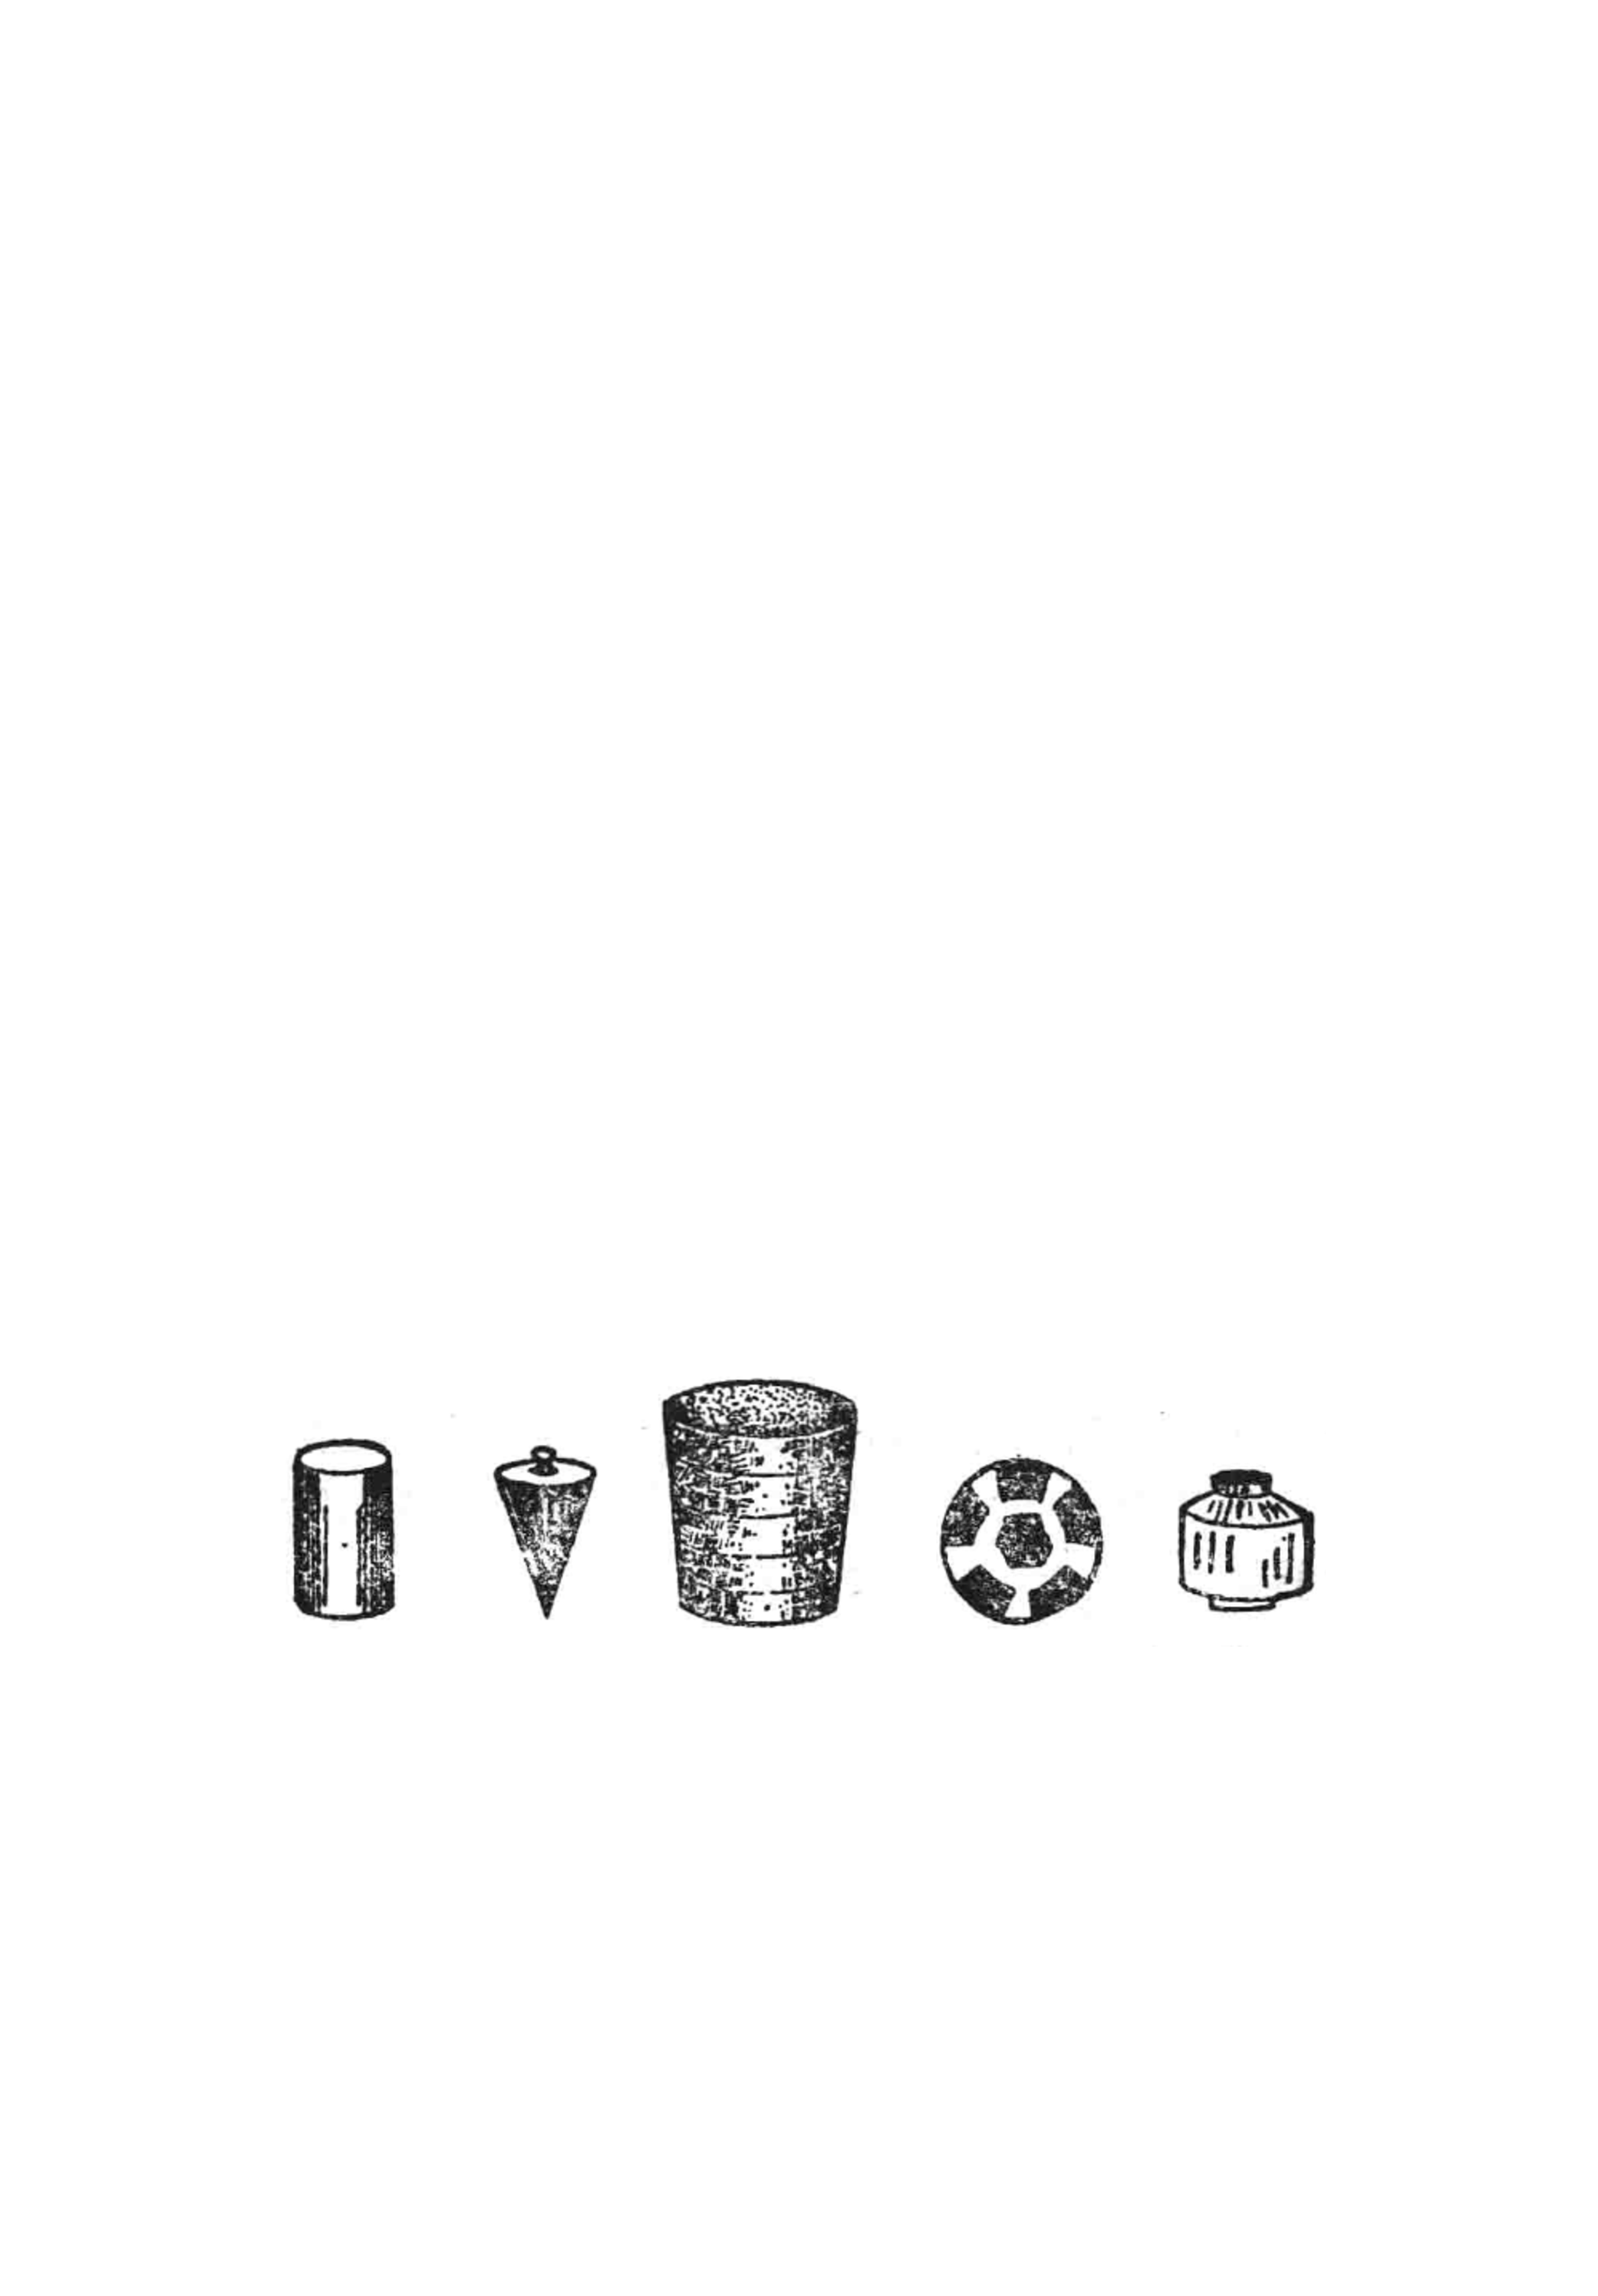
\includegraphics[scale=.5]{fig/2-44.pdf}
    \caption{}
\end{figure}

它们的表面至少有一部分是曲面，这种曲面不是任意的形状而是一种旋转面.


一条平面曲线（包括直线）绕它所在的平面内的一条定直线旋转一周，所形成的曲面叫做\textbf{旋转面}. 这条定直线叫做
旋转轴，无论转到什么位置，这条曲线都叫做旋转面的\textbf{母线}.

如果母线是与旋转轴平行的直线，所形成的旋转面叫圆柱面（图2.45甲），如果母线是和旋转轴斜交的直线，所形成的旋转面叫圆锥面（图2.45乙），这时母线和轴的交点叫做圆锥面的顶点，如果母线是半圆且旋转轴是它的直径，所形成的旋转面就是球面（图2.45丙）．如果一个圆，绕同一平面内与它不相交的一条直线旋转一周，那么形成的旋转面叫做\textbf{环面}（图2.45丁）．

\begin{figure}[htp]
    \centering
\begin{tikzpicture}
\begin{scope}
\draw[thick](0,2) ellipse (1 and .5);
\draw[thick](-1,2)--node[left]{$\ell$}(-1,0);
\draw[thick](1,2)--(1,0);
\draw[thick](1,0) arc [start angle =0, end angle =-180, x radius =1, y radius=.5]; 
\draw[dashdotted](0,-1)node[below]{甲}--(0,3)node[above]{$a$};
\end{scope}
\begin{scope}[xshift=2.8cm]
\draw[thick](0,2) ellipse (.58 and .3);
\draw[thick](-.6,2)--(1,0);
\draw[thick](.6,2)--node[left]{$\ell$}(-1,0);
\draw[thick](1,0) arc [start angle =0, end angle =-180, x radius =1, y radius=.5]; 
\draw[dashdotted](0,-1)node[below]{乙}--(0,2.8)node[above]{$a$};

\tkzDefPoints{-.6/2/A, 1/0/B, .6/2/A1, -1/0/B1}
\tkzInterLL(A,B)(A1,B1)
\tkzGetPoint{O}
\tkzLabelPoints[right](O)
\end{scope}
\begin{scope}[xshift=5.5cm]
    \draw[dashdotted](0,-1)node[below]{丙}--(0,2.5)node[above]{$a$};
\draw[thick](0,1) circle (1);
\draw[thick](1,1) arc [start angle =0, end angle =-180, x radius =1, y radius=.4]; 
\draw[dashed](1,1) arc [start angle =0, end angle =180, x radius =1, y radius=.4]; 
\node at (.9,1.8){$\ell$};
\node at (0,1)[left]{$O$};
\tkzDefPoints{0/1/O}
\tkzDrawPoints(O)
\end{scope}
\begin{scope}[xshift=9cm]
    \draw[thick](0,1) ellipse (1.5 and .7);
    \draw[thick](0,1) ellipse (.7 and .3);
    \draw[dashdotted](0,-.5)--(0,2.5)node[above]{$a$};
   \node at (0,-1)[below]{丁};
\draw[thick](0,.7) arc [start angle =90, end angle =-90, x radius =.1, y radius=.2]; 
\draw[dashed](0,.7)  arc [start angle =90, end angle =270, x radius =.1, y radius=.2]; 
\node at (0.3,.5)[]{$\ell$};

\end{scope}    
\end{tikzpicture}
    \caption{}
\end{figure}


什么是旋转体呢？一个封闭的平面图形，绕它所在平面内的一条定直线旋转一周，形成的旋转面所围成的几何体叫做\textbf{旋转体}，这条定直线叫做旋转体的\textbf{轴}.

前面我们提到的圆钢、铅锤、粮囤、排球、墨水瓶、轮胎等都是旋转体的形象.

\subsection*{2.4 练习}
\begin{enumerate}
\item 举出一些旋转面和旋转体的实例.
\item 圆柱面、圆锥面的母线是直线，还是曲线，还是线段？
它们和旋转轴的位置关系如何？
\item 球面的母线是什么形状的曲线？
\item 旋转体与旋转面有什么关系？
\end{enumerate}
